%% LyX 2.1.3 created this file.  For more info, see http://www.lyx.org/.
%% Do not edit unless you really know what you are doing.
\documentclass[twocolumn,english]{article}
\usepackage[LGR,T1]{fontenc}
\usepackage[latin9]{inputenc}
\usepackage{geometry}
\geometry{verbose,tmargin=2cm,bmargin=2cm,lmargin=1cm,rmargin=1cm,columnsep=1cm}
\usepackage{color}
\usepackage{array}
\usepackage{rotfloat}
\usepackage{multirow}
\usepackage{amsmath}
\usepackage{amssymb}
\usepackage{graphicx}
\PassOptionsToPackage{normalem}{ulem}
\usepackage{ulem}

\makeatletter

%%%%%%%%%%%%%%%%%%%%%%%%%%%%%% LyX specific LaTeX commands.
\DeclareRobustCommand{\greektext}{%
  \fontencoding{LGR}\selectfont\def\encodingdefault{LGR}}
\DeclareRobustCommand{\textgreek}[1]{\leavevmode{\greektext #1}}
\DeclareFontEncoding{LGR}{}{}
\DeclareTextSymbol{\~}{LGR}{126}
%% Because html converters don't know tabularnewline
\providecommand{\tabularnewline}{\\}
%% A simple dot to overcome graphicx limitations
\newcommand{\lyxdot}{.}


\makeatother

\usepackage{babel}
\begin{document}

\title{\textcolor{black}{Automated Dune Crestline Detection}}


\author{\textcolor{black}{David Leblanc}}


\date{\textcolor{black}{10/08/2015}}
\maketitle
\begin{abstract}
\textcolor{black}{TODO}
\end{abstract}

\section{\textcolor{black}{Introduction}}

\textcolor{black}{TODO}


\section{\textcolor{black}{Previous Work}}


\subsection{\textcolor{black}{Dune Pattern Studies}}

\textcolor{black}{In \cite{Kocurek_Ewing}, an explanation of how
dune-field patterns emerge and addresses the degree of complexity
from the standpoint of self-organizing system. Dune patterns are classified
into two basic categories: simple or complex. According to this paper,
a simple pattern is defined as having a single pattern type. Complex
patterns are said to potentially have multiple spatially superimposed
pattern types. Simple patterns trend towards a better ordering, so
long as the wind regime remains constant. Changes in the trend of
wind pattern will cause reorientation. Complex patterns can then be
interpreted as the superposition of many generations of wind regimes. }

\textcolor{black}{Complexity can be measured using pattern analysis,
measuring parameters such as the crest length, orientation, spacing,
defect density, and other properties. These properties would be very
useful information to extract for the dune detection. Finding crest-lines
can help us identify the patterns, extracting meanful data such as
junctions, terminations, mergers, linking, and other interesting processes
explained in \cite{Kocurek_Ewing}.}

\textcolor{black}{In later work, \cite{Ewing_Peyret_Kocurek_Bourke}
studied the dune field pattern formations on the north polar region
of Mars. These dunes are thought to be mostly inactive, with relative
no movement over a period of 4 to15 martian years. The reason this
region is interesting is because there are two nearly orthogonal crestline
orientations present in the region. This complex system of superposition
of multiple patterns in this example showcase a set of }\textcolor{black}{\emph{primary}}\textcolor{black}{{}
and }\textcolor{black}{\emph{secondary}}\textcolor{black}{{} crestlines
which would be valuable data to automatically segment. The }\textcolor{black}{\emph{primary}}\textcolor{black}{{}
dunes are the largest-scale dunes, extend over the entire lenght of
the image set, and contain many }\textcolor{black}{\emph{Y }}\textcolor{black}{junctions,
an indication of well-organized linear dunes. In contrast, }\textcolor{black}{\emph{secondary}}\textcolor{black}{{}
dunes are rounded, have least defined features, and are perpendicular
to the main primary crestlines.}

\textcolor{black}{Other interesting features are the so-called }\textcolor{black}{\emph{Slipfaces}}\textcolor{black}{.
These typically appear along the }\textcolor{black}{\emph{primary}}\textcolor{black}{{}
crestlines, in areas of intersection with the }\textcolor{black}{\emph{primary}}\textcolor{black}{{}
and }\textcolor{black}{\emph{secondary}}\textcolor{black}{{} crestlines.
Another feature are the }\textcolor{black}{\emph{Wind Ripples}}\textcolor{black}{.
The ripples are present on the surface of most dunes with the exception
of }\textcolor{black}{\emph{slipfaces}}\textcolor{black}{. To detect
these types of features, a higher resolution image is a required,
as those types of features are very small compared to the scale of
the }\textcolor{black}{\emph{primary}}\textcolor{black}{{} and }\textcolor{black}{\emph{secondary}}\textcolor{black}{{}
dunes. }\textcolor{black}{\emph{Interdune Areas}}\textcolor{black}{{}
are features specific to the area studied in \cite{Ewing_Peyret_Kocurek_Bourke},
have a polygonal shape, and are indicative of ice.}

\textcolor{black}{The rest of the paper describes an in depth statiscal
analysis of the features to compute the flow fields and understand
the geomorphic relationships which are present in the area}\footnote{\textcolor{black}{The paper \cite{Ewing_Peyret_Kocurek_Bourke} provides
a lot of interesting and valuable information which can be used to
understand the application of automatic dune detection. If these features
can be extracted, it would be interesting to see if we can do a similar
statistical analysis based on the results presented. The next step
would be to retrieve the HiRISE dataset and their data or ground truth
to compare. }}\textcolor{black}{.}

\textcolor{black}{In the most recent work, \cite{Multi_spatial_analysis_aeolian_dune_field_patterns}
study the aeolian dune-fields at different scales. Scale is an important
factor to consider because aeolian dune-fields patterns can vary over
a wide range of scales, both spatially and temporally. Being able
to measure the change of scale over time is important in order to
investigate the environmental conditions of the studied region. Aeolian
dunes are developped typically in transitions from sand patches, to
proto-dunes, to dunes, to dune-field patterns. Complex dune patterns
are usually a juxtaposition of simple dune patterns are multiple scales.
To summarize, being able to detect the crestlines and other types
of features at multiple scales is invaluable.}

\textcolor{black}{In other related work, \cite{Application_spatial_cross_correlation_detection_submarine_dunes}
studied the migration of submarine sand dunes. The dataset used in
this paper includes digital terrain models (DTMs) retrieved from high-density
multibeam echosounders (MBES) taken of submarine sand dunes along
the coast of New Brunswick. In order to measure the migration of these
types of dunes, the motion was measured by simply subtracting the
DTMs from sequences over time. The implementation uses a simple cross-correlation
to find similarities from one set to the next. From the correlation
matches found, the migration vector can be computed. The migration
data processing can extract the flow fields of the dunes.}


\subsection{\textcolor{black}{Image Processing}}


\subsubsection{\textcolor{black}{Filtering}}

\textcolor{black}{There are many common filtering approaches used
in image processing and computer vision applications. In this application,
satelite images of sand dunes may include various ammounts of noise.
In order to improve the dune detection algorithms, the goal of filtering
is to filter out the noise while preserving or enhancing the necessary
features such as the crest-line edges.}

\textcolor{black}{In \cite{Bilateral-filtering-gray-color-images},
the bilateral filter is proposed, which allows flat noisy regions
to be filtered while preserving strong edges. Bilateral filtering
is a simple non-iterative algorithm for filtering out noise.}


\subsubsection{\textcolor{black}{Illumination Normalization}}

\textcolor{black}{Illumination normalization is a process in which
the image illumation is made to be more evenly distributed accross
the image, to make the illumination invariant in conditions of varying
lighting. This processing is most commonly used in face detection
or recognition applications. In \cite{Illumination_normalization_based_on_2d_gaussian_model},
a Gaussian illumination model is used to stretch the contrasts of
darker areas. The process involves using a Quadtree method to divide
the image into sub regions to find dark areas. The areas that meet
these requirements are processed with the Gaussian illumination model
to brighten them up, which evens out the illumination. Applying this
normalization significantly improves performance of face recognition.}

\textcolor{black}{In a similar approach \cite{Illumination_normalization_for_image_restoration_using_modified_retinex_algorithm},
the authors use a modified retinex algorithm to restore poorly illuminated
areas of an image. According to Lambertian reflectance theory, images
consist of two components, reflectance and illumination. If an image
contains a set of small scale features, and large scale features,
and illumination is only applied to the large-scale set, then the
small scale features can be preserved. In this approach, the normalization
is applied to small-scale and large-scale features independently.
The Single Scale Retinex process is applied to the image to seperate
the reflectance (small scale) and illumination (large scale). After,
images are thresholded and histogram equalization is applied, which
spreads out intensity values of darker areas of the image.}

\textcolor{black}{In a remote sensing application, \cite{Illumination_normalization_among_multiple_remote_senging_images},
illumination normalization in the gradient domain and using singular
value equalization. According to the authors, the gradient domain
image enhancement process can compress the dynamic range of images,
increase contrast, and enhance fine details in darker regions. The
goal of singular value equalization is to make all images in a specific
set to have similar mean intensity value. Some images may have a lower
or higher mean intensity. By using SVE, the pixels can be processed
to achieve a mean closer to the target intensity, therefore normalizing
illumination accross a set of images. The drawback of this method
is that multiple images of the same or similar scenes are required.}


\subsubsection{\textcolor{black}{Edge and Line Detection}}

\textcolor{black}{The Canny edge detector is a well known and used
method to retrieve important edge features from an image. In \cite{Canny_edge_detection_enhancement_scale_multiplication},
enhancement to the method is proposed by analysing the responses of
detection at two scales. The benefits of this technique are better
localization in images with larger amounts of noise, at the cost of
a slightly lower detection rate. Overall the performance of the Canny
operator is improved by using multiple scales.}

\textcolor{black}{The Canny detector is further improved in \cite{Runway_detection_tracking_unmanned}
for a runway detection application for unmanned aerial vehicles. The
main contribution of this paper is the use the Canny operator combined
with a mean filter, and using the Hough Transform to track runways.
The advantages o f the mean filtering is that it filters out noise,
preserves edges (better than a traditional Gaussian filter), and makes
the image less fuzzy. To solve the problem of the dual threshold of
the Canny operator, the proposed method is to compute the thresholds
dynamically based on averages.}

\textcolor{black}{In \cite{Improved_Canny_Edge_Detection}, an improved
implementation of the popular Canny edge detector is proposed. According
to the authors, the traditional Canny algorithm suffers from two main
problems: the gradient calculation is sensitive to noise and the use
of the fixed double threshold may not be suitable for images with
high gradient variability. The main flaw in the gradient calculation
has to do with the inequality of the edge detection in darker versus
brighter regions. For the parameter selection of the double threshold,
the paper propose chosing the high and low thresolds from the computed
mean and standard deviation of the gradient magnitudes.}

\textcolor{black}{A line detection and image enhancement has been
proposed in \cite{Robust_Faint_Line_Detection_Enhancement_Algorithm},
for a digital image restoration of heritage art application. The images
worked with have been deteriorated over time, and contain many cracks,
faint lines, and broken stroke. The goal of this is to remove unwanted
edges, and enhance the desired edges. The approach is implemented
in three basic steps: Initial line detection with non-maxima suppression,
true line detection using anisotropic refinement, and noise reduction.}

\textcolor{black}{The initial step is to perform correlation convolving
the image with some sort of edge detecting mask, rotated at different
orientations, and retrieving the maximum response for the orientation
for each pixel. The paper claims this produces a sharper and more
reliable edge map, which is then filtered using non-maxima supression.
This process preserves strong lines while removing texture lines.
The image is the binarized to remove all remaining weak edges, and
only allowing strong edges to remain. The smoothing is applied to
the original based on the processing done, smoothing out weak edges,
while not smoothing strong true edges.}

\textcolor{black}{In a similar approach, \cite{Image_Edge_detection_Rotating_Kernel_Transformation}
use rotating edge detection kernels and fuse the responses from the
operations. What determines what an edge is a location and a direction,
as a non-edge point such as a flat area or noise, which has no specific
direction. Following this principle, the response in on direction
should be higher than in the other directions. For a non-edge, the
responses in each of the directions are similar. Therefore computing
the mean and standard deviation of each of the kernel responses can
help resolve edge versus non edge pixels. The results obtained from
this process shows promising results when applied to noisy images}\footnote{\textcolor{black}{The approach proposed in \cite{Image_Edge_detection_Rotating_Kernel_Transformation}
has definite potential for improved edge detection applied to dune
crestline detection. It also has potential for improvement of the
method itself}}\textcolor{black}{.}

\textcolor{black}{An interesting alternative to the classical Hough
transform is presented in \cite{Automated_cable_tracking_sonar_imagery}
in an application inspection or maintenance of underwater cable components.
The paper discusses image processing techniques to extract linear
features in cluttered and noisy images. After applying some anisotropic
filtering to remote high frequency noise, edges and lines are detected
on the sonar based images. To detect potential linear features, they
use a Phase Congruency detector}\footnote{\textcolor{black}{The Phase Congruency detector requires more research
to determine what type of features can be extracted from it.}}\textcolor{black}{. The Hough transform is then used to find linear
features, and some criterias are determined to reject false positives
and preserve true positives.}


\subsubsection{\textcolor{black}{Edge Linking}}

\textcolor{black}{In \cite{Edge_linking_using_geodesic_distance_neighborhood_information},
an edge linking approach is proposed which using local neighborhood,
using geodesic distance (as opposed to the common Euclidean distance
measure) between edge candidates. When calculating the direction of
edge end points, typically eight directions are used, which introduces
error. To address this \cite{Edge_linking_using_geodesic_distance_neighborhood_information}
define a windows size based on the maximum allowable edge gap, and
fit a line to the edges, which allows a full range of directions to
be accounted for. The geodesic distance measurement is not only based
on euclidean distance but also on intensity values of the image, which
reportedly gives better results.}


\subsection{\textcolor{black}{Pattern Recognition}}


\subsubsection{\textcolor{black}{Perceptual Grouping}}

\textcolor{black}{The concept of tensor voting introduced in (REFERENCE
NEEDED!!!).}

\textcolor{black}{In \cite{Probabilistic-tensor-voting-robust-perceptual-grouping},
a tensor voting approach is used to perform perceptual grouping on
noisy data. The approach extends the standard tensor voting using
Bayesian probilities. The Bayesian framework has added benefits of
reducing the learning variance of the perceptual grouping task. Another
contribution of this paper is the use of a 2nd order tensor and two
types of polarity vectors to handle both outlier and inlier noise.
The approach also is able to process all types of geometric structures.
For probabilistic tensor voting, the voting procedure uses random
vector with a given standard deviation. It uses three layers of voting:
sparse ball vote, sparse stick vote, and revised stick vote, where
the goal is to change the positions of each token based on a random
vector.}


\subsubsection{\textcolor{black}{Watershed Segmentation}}

\textcolor{black}{The Watershed Transform is a well know algorithm
for segmenting meaningful regions from an image. The main benefit
of the watershed technique as opposed to method, such as edge-based
detection, is that the watershed produces closed boundaries, which
allows contours to be detected. An overview of the Watershed algorithm
is presented in \cite{Watershed-transform-definition-algorithms-parallelization-strategies}}\footnote{\textcolor{black}{This paper still needs to be read}}\textcolor{black}{.}

\textcolor{black}{In \cite{Image_segmentation_using_texture_gradient_based_watershed_transform},
segmentation is achieved using the watershed transform from texture
gradients. The texture gradients are retrieved using various wavelet
transforms.}

\textcolor{black}{Similarly, in \cite{Watershed-based-textural-image-segmentation},
an approach to texture segmentation is proposed. When applied to textures,
the watershed algoritm tends to over-segment a texture into small
homogeneous sub-texture regions. Therefore, a texture can be determined
to be set of texture segments. The texture sub-regions can be merged
using a clustering algorithm. A wavelet transform is used to characterize
the irregular shaped segment regions, which are used to cluster similar
groups of sub-textures.}

\textcolor{black}{Another approach used in the Watershed algorithm
is based on markers. The desired regions to segment can be extracted
using some known feature which gets marked on the image. In \cite{Fingerprint-pore-extraction-based-marker-controlled-watershed-segmentation},
this concept is applied to a fingerprint pore extraction application.
Marker based segmentation has been shown to be robust for segmentations
problems where the objects are closed contours with boundaries being
ridges. In this application, the watershed transform is applied to
the gradient image of the fingerprints, and the regional minimas are
computed to obtain the markers, then compute the watershed transform
based on the markers.}

\textcolor{black}{In \cite{Detection-breast-tumor-candidates-using-marker-controlled-watershed-segmentation},
the watershed segmentation is applied to a breast tumor detection
application.}


\subsection{\textcolor{black}{Automated Feature Detection}}

\textcolor{black}{In \cite{Extraction_roads_multispectral_imagery},
a semi-automated method for extracting roads from aerial or satellite
images is proposed. The purpose of this paper is to localize roads
from higher resolution images, using some form of segmentation. The
proposed method is semi-automated because a user must provide and
initial seed point, onto which a region growing algorithm is applied
to extract the road. }

\textcolor{black}{A level set method is applied to evolve the boundary
of the road region, which can better handle noise and multiple road
mergers. The boundary for the desired region is based on a speed function,
which is designed based on uniformity, texture, and contrast properties.
Once the regions have been extracted, the centerlines of the roads
are estimated using a skeletonization procedure, with junction analysis
to ensure that intersections are properly handled}\footnote{\textcolor{black}{The skeletonization procedure used in \cite{Extraction_roads_multispectral_imagery}
may be useful for extracting the dune crestlines and junction points
from segmented dune regions.}}\textcolor{black}{.}

\textcolor{black}{In \cite{Extracting_ocean_surface_feature_modis},
linear features of internal waves are extracted using a technique
called }\textcolor{black}{\emph{Multiscale Retinex }}\textcolor{black}{(MSR)
feature extraction}\footnote{\textcolor{black}{Although the problem set in \cite{Extracting_ocean_surface_feature_modis}
is different, there appears to be significant overlap and comparison
between dune crestline detection and oceanic internal wave detection.}}\textcolor{black}{. The oceanic internal waves are typically generated
from many sources such as tidal currents, ocean frontal boundaries,
and other atmospheric conditions. The MSR is an image processing technique
that provides consistency and dynamic range compression accross an
image with poor contrast. The paper discusses the use both the Wavelet
Transform Modulus Maxima (WTMM) and the Canny edge detector, which
turned out to have superior performance.}

\textcolor{black}{There has been some work done in automated dune
detection. In \cite{BandeiraMarques}, a supervised learning approach
is used, training classifiers such as Support Vector Machine and Random
Forests to detect dune structures on Mars. The method proposed in
this paper is to classify small (40 by 40 pixels) cells in a quantized
image grid. In each cells features are computed based on the image
gradients, using both phase and magnitude. In order to classify a
cell as either a dune or not a dune, the features of both the cell
and the cell's neighboring cells are used. The features extracted
are then used to train the machine learning method, which is used
to then predict if a cell is a dune.}

\textcolor{black}{Although this type of method has typically shown
very good results, there are a few drawbacks with using supervised
learning approaches. These types of methods usually require a fairly
large labelled dataset which may not always be available. Anytime
a dataset is constructed for this purpose, it is important to provide
a large number of examples of different types of dunes, in order to
get a robust representation of the problem set. In \cite{BandeiraMarques},
230 labelled images were used to train and test the method, and have
a decent representation of various dune types. Another drawback of
this approach is the use of cells, for which fixed-sized cells may
not be scale invariant. Also, quantizing an image into largers cells
will affect localization accuracy of the dunes. If the application
requires higher localization accuracy, this type of surpervised learning
approach may not be suitable.}


\subsection{\textcolor{black}{Automated Dune Detection}}

\textcolor{black}{In \cite{Automated-mapping-linear-dunefield-morphometric-parameters},
an automated extraction of dune features is proposed. In this approach,
the authors claim that the Canny edge detector provided poor results,
and the sobel operator generated more consistant results. The gradient
magnitude of the Sobel operator is used to threshold out the weaker
edges. The use of a histogram to compute the orientations of the gradients
was found to have a bimodial distribution, with one of the modes being
the dune edges. Dune candidates are determined based on their gradient
magnitude which filter out weaker candidates unless they are near
strong candidates.}


\section{\textcolor{black}{Methodology}}


\subsection{\textcolor{black}{Dune Detection}}


\subsubsection{\textcolor{black}{\label{sub:Method-=0000231:-Adaptive}Method \#1:
Adaptive threshold and contour detection}}


\paragraph{\textcolor{black}{Adaptive Threshold Image Process:}}

\textcolor{black}{Dune crest images typically have a shaded and a
light side. Depending on the conditions and image quality, the actual
edge or dune crest line may not be clearly defined. Some image processing
typically improves the quality and allow the extraction of the dune
crest lines.}

\textcolor{black}{Many approaches revolve around edge detection, but
because the conditions and image quality can vary, edges may not be
accurately extracted. In this approach, we use a thresholding method
to extract the light side of a dune. Using a fixed threshold may not
be sufficient to extract the dunes since the illumination across an
image is usually not uniform. An adaptive threshold can be a useful
tool to threshold an image with non-uniform illumination. An example
of this type of thresholding is shown in Figure \ref{fig:AdaptiveThreshold1}.}

\textcolor{black}{}
\begin{figure}
\begin{centering}
\textcolor{black}{\includegraphics[scale=0.23]{\string"Figures/Datasets/Kalahari 3 image\string".jpg}}
\par\end{centering}

\begin{centering}
\textcolor{black}{\includegraphics[scale=0.23]{\string"Figures/Kalahari 3 image.jpg_result\string".jpg}}
\par\end{centering}

\textcolor{black}{\protect\caption{\label{fig:AdaptiveThreshold1}Example of an adaptive thresholding
method applied on a dune crest image with poor illumination and contrast.}
}
\end{figure}



\paragraph{\textcolor{black}{Dune Crest Line Extraction:}}

\textcolor{black}{Once the image has been preprocessed, the bright
regions can extracted from the resulting binary image. As shown in
figure \ref{fig:AdaptiveThreshold1}, the bright regions shown consist
of the sun illuminated side of the dunes and some noise. }

\textcolor{black}{From the regions, contours can be extracted, which
can be filtered by size of the region. Smaller regions are considered
as noise, and can be rejected from the potential dune candidates.
The remaining region contours are used as potential candidates for
dune crest lines. From the coutours, figure \ref{fig:AdaptiveThreshold1}
shows that typically one of the edges of the contour is located very
nearly on the dune crest line. On the opposite side of the region
is essentially the base of the dune. Figure \ref{fig:Contour-extraction-from}
shows the results of the extracting the contours from the processed
image.}

\textcolor{black}{}
\begin{figure}
\begin{centering}
\textcolor{black}{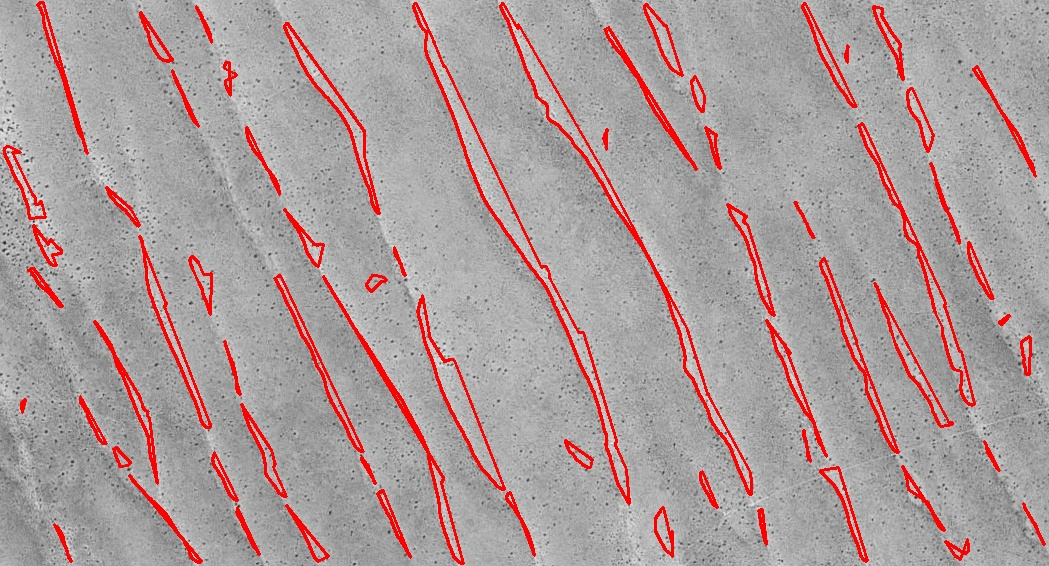
\includegraphics[scale=0.23]{Figures/ContourResults}}
\par\end{centering}

\textcolor{black}{\protect\caption{\label{fig:Contour-extraction-from}Contour extraction from binary
processed image}
}

\end{figure}


\textcolor{black}{Because the regions tend to be noisy, the contours
are therefore smoothed using a Gaussian kernel, define as:}

\textcolor{black}{
\[
G\left(i\right)=\frac{1}{\sqrt{2\pi}\sigma}e^{\frac{-i^{2}}{2\sigma^{2}}}
\]
}

\textcolor{black}{The Gaussian kernel is convolved on the contour,
which a collection of two dimentional points (x,y). The result of
this convolution is a smoother contour which can be more reliably
used as a dune crest line candidate.}

\textcolor{black}{Typically, the dune crest lines are located on an
area in the image where the derivatives are larger, or consistant
along the edge of the dune. For each contour, the average magnitude
}\textcolor{black}{\emph{\textgreek{m}}}\textcolor{black}{{} of the
derivative }\textcolor{black}{\emph{\textgreek{d}}}\textcolor{black}{(}\textcolor{black}{\emph{i}}\textcolor{black}{)
of the image in the }\textcolor{black}{\emph{x}}\textcolor{black}{{}
and }\textcolor{black}{\emph{y}}\textcolor{black}{{} directions is computed.
Then, for each point within a contour compares its derivative with
}\textcolor{black}{\emph{K}}\textcolor{black}{{} neighbor's gradient
magnitudes. Dune crest line candidate points will tend to have neighbors
with similarly and consistantly high gradients. To determine if a
point }\textcolor{black}{\emph{P}}\textcolor{black}{(}\textcolor{black}{\emph{i}}\textcolor{black}{)
on a contour belongs on the dune crest line, we use the following
criteria}

\textcolor{black}{
\[
P\left(i\right)=\begin{cases}
1 & \phi(i)\geq r\\
0 & otherwise
\end{cases}
\]
}

\textcolor{black}{where}

\textcolor{black}{
\[
\phi(i)=\frac{\sum_{k=0}^{K}\begin{cases}
1 & \delta\left(k\right)\geq\mu\\
0 & \delta\left(k\right)<\mu
\end{cases}}{K}
\]
}

\textcolor{black}{and $0<r\leq1$, which is the ratio of how many
strong consistant edges to neighbors around a point }\textcolor{black}{\emph{i}}\textcolor{black}{{}
on the contour. Typically, }\textcolor{black}{\emph{r}}\textcolor{black}{{}
would be larger than 0.5, which means most of the neighbors of a point
most have strong edges for a point to be considered a dune crest line
candidate. The parameter }\textcolor{black}{\emph{r}}\textcolor{black}{{}
can be fine tune to allow more or less points to fit the criteria.
This method will group common contour points based on gradient magnitude.}

\textcolor{black}{Once the dune crest line candidates on the contour
have been extracted, the contour can be split into contiguous crest
line segments. Some further processing can be applied to the segments,
such as filtering out smaller or less significant segments (potential
false positives). More work needs to be done in this area.}


\subsubsection{\textcolor{black}{\label{sub:Method-=0000232:-Unsupervized}Method
\#2: Unsupervized Edge-based line detection}}


\paragraph{\textcolor{black}{Edge Detection Image Processing:}}

\textcolor{black}{This approach is based on the gradient information
detect on the image. Dune crestlines typically have relatively large
gradient magnitudes. There are a few challenges with extracting edges
of the dune satelite images:}
\begin{enumerate}
\item \textcolor{black}{Images tend to be noisy and very textured, which
results in many edges of varying orientations and magnitudes.}
\item \textcolor{black}{Many of the stronger edges may not necessarily be
the crestlines themselves. Generally, dunes cast relatively large
shadows which themselves produce relatively strong edges.}
\item \textcolor{black}{Determining the parameters and appropriate scale
for the parameters of the edge detector can be sensitive and affect
detection rates.}
\end{enumerate}
\textcolor{black}{To address these concerns, the Canny edge detector
is used along side some of the techniques inspired from \cite{Improved_Canny_Edge_Detection}
and \cite{Runway_detection_tracking_unmanned}. First, in order to
reduce the amount of noise in the images, both a median and Gaussian
filtering is applied to the image. The reasoning for the median filter
removes small speckles (which for dune images may be small bushes
or other contrasting features found in the images) while preserving
major edge gradients. The Gaussian filter will then smooth out the
gradient magnitudes and even out the image.}

\textcolor{black}{Another important pre-processing step is to apply
histogram equalization (REFERENCE NEEDED) to the image. Histogram
equalization is important because it stretches the contrast which
is crucial to feature extraction in dune-field images, which tend
to have poor contrast. This in turns also helps in the extraction
of edges, and improves determination of the dominant gradient orientation.}

\textcolor{black}{Once the image has been pre-processed, the Canny
edge detector is used to recover the potential crestline candidates.
To overcome the parameter selection of the high and low threshold,
the mean gradient }\textcolor{black}{\emph{\textgreek{m} }}\textcolor{black}{and
standard deviation }\textcolor{black}{\emph{\textgreek{sv}}}\textcolor{black}{{}
is computed over the entire image. The high and low thresholds are
determined as follows:}

\textcolor{black}{
\[
T_{high}=\mu+q\centerdot\sigma
\]
}

\textcolor{black}{
\[
T_{low}=\frac{T_{high}}{2}
\]
}

\textcolor{black}{where }\textcolor{black}{\emph{q}}\textcolor{black}{{}
is so factor which can be determined based on the problem set. This
makes the threshold parameter less sensitive to fixed threshold problems.
The result of the Canny edge detector after filtering are displayed
in figure \ref{fig:Canny-edge-detector}.}

\textcolor{black}{}
\begin{figure}
\begin{centering}
\textcolor{black}{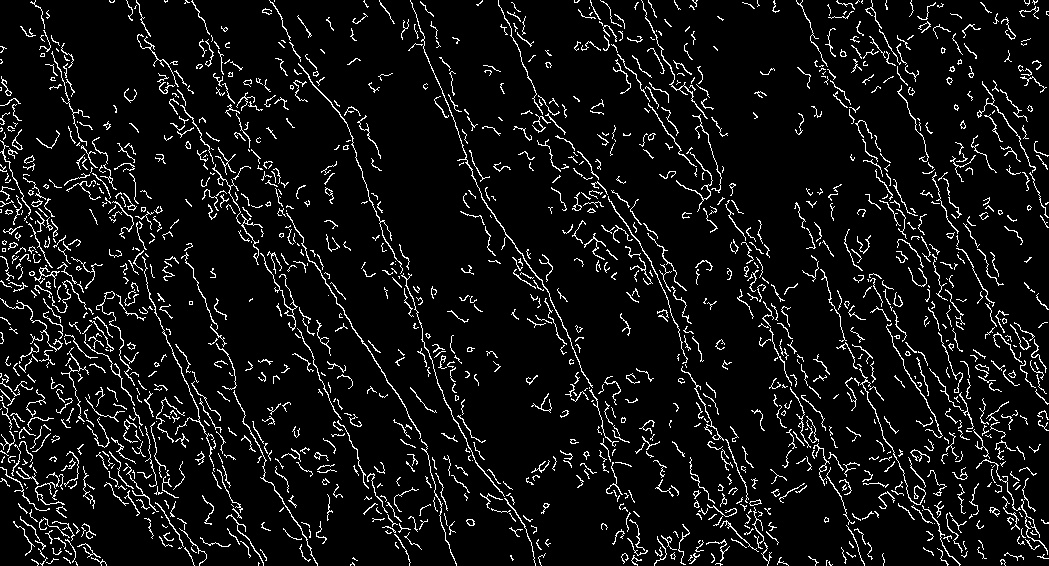
\includegraphics[scale=0.23]{Figures/M2_edge_map}}
\par\end{centering}

\textcolor{black}{\protect\caption{\label{fig:Canny-edge-detector}Canny edge detector after median and
Gaussian filtering of the Kalahari dune image.}
}
\end{figure}



\subsubsection*{\textcolor{black}{Unsupervised Crestline Detection from Detected
Edges}}

\textcolor{black}{Many of the edges provided in the edge detection
step are noise, shadows, and non crestline textures. Crestlines all
have one feature in common: all of their gradient have relatively
similar orientations. Dune crests typically appear to have larger
gradient magnitures relative to other noisy edges or texture (but
this may not always be the case). To help solve this issue, as mentionned
above, using histogram equalization can help normalize edges and improves
calculation of the dominant orientation of the edges.}

\textcolor{black}{Similarly, because of the position at which the
sun, edges generated from the shadows of the dunes will also have
similar orientations within themselves. Given these properties, there
should be a clear deliniation between crestline edges, and non-crestline
edges.}


\paragraph*{\textcolor{black}{\uline{Using KMeans}}\textcolor{black}{:}}

\textcolor{black}{Resolving these differences by grouping similar
edges together can be achieved by clustering the gradients. There
have been many approaches to clustering (REFERENCES NEEDED HERE???),
but the most common is the K-Means algorithm. The benefits of using
a clustering algorithm is that it is unsupervised, so that the differences
should form themselves from the edge data itelf.}

\textcolor{black}{Typically, the main parameter that is required for
K-Means is the value }\textcolor{black}{\emph{K,}}\textcolor{black}{{}
which is the number of clusters. In this problem set, the goal is
to seperate the crestline group from all other non-crestline edges.
Therefore, the parameter is simply set to $K=2$, to seperate the
gradients into two distinct groupings}\footnote{\textcolor{black}{So far, only using two clusters has been investigated.
Using more clusters may have more valuable information and better
seperation.}}\textcolor{black}{.}

\textcolor{black}{In order to get normalized results for the clustering
algorithm, the gradients themselves are normalized. To normalize the
gradients, the average gradient magnitude of the detected edges is
computed as:}

\textcolor{black}{
\[
\bar{\mu}=\frac{\sum_{i=0}^{P}\sqrt{\delta_{x_{i}}^{2}+\delta_{y_{i}}^{2}}}{P}
\]
}

\textcolor{black}{where }\textcolor{black}{\emph{P}}\textcolor{black}{{}
is the total number of detected edges from the Canny edge detector,
$\delta_{x_{i}}$ and $\delta_{y_{i}}$ are the }\textcolor{black}{\emph{x}}\textcolor{black}{{}
and }\textcolor{black}{\emph{y}}\textcolor{black}{{} gradient component
of the }\textcolor{black}{\emph{i}}\textcolor{black}{th point. Each
gradient is then normalized by dividing by the average magnitude $\bar{\mu}$.}

\textcolor{black}{
\[
\dot{\delta}\left(x_{i},y_{i}\right)=\left(\frac{\delta_{x_{i}}}{\bar{\mu}},\frac{\delta_{y_{i}}}{\bar{\mu}}\right)
\]
}

\textcolor{black}{The set of normalized gradient vectors are then
clustered using the K-Means algorithm with $K=2$. In Figure \ref{fig:Results-of-K-Means},
the results of the clustering method are shown. The blue points are
gradient vectors which potentially belong to the dune crestline. Studying
the points, we notice that there is a skew towards the stronger edges
in the blue cluster, which we will call the dominant cluster. This
is determined by computing the centroids of each cluster. The cluster
with the larger overall gradient magnitude is therefore assumed to
be the set which contains the crestline points.}

\textcolor{black}{}
\begin{figure*}
\begin{centering}
\textcolor{black}{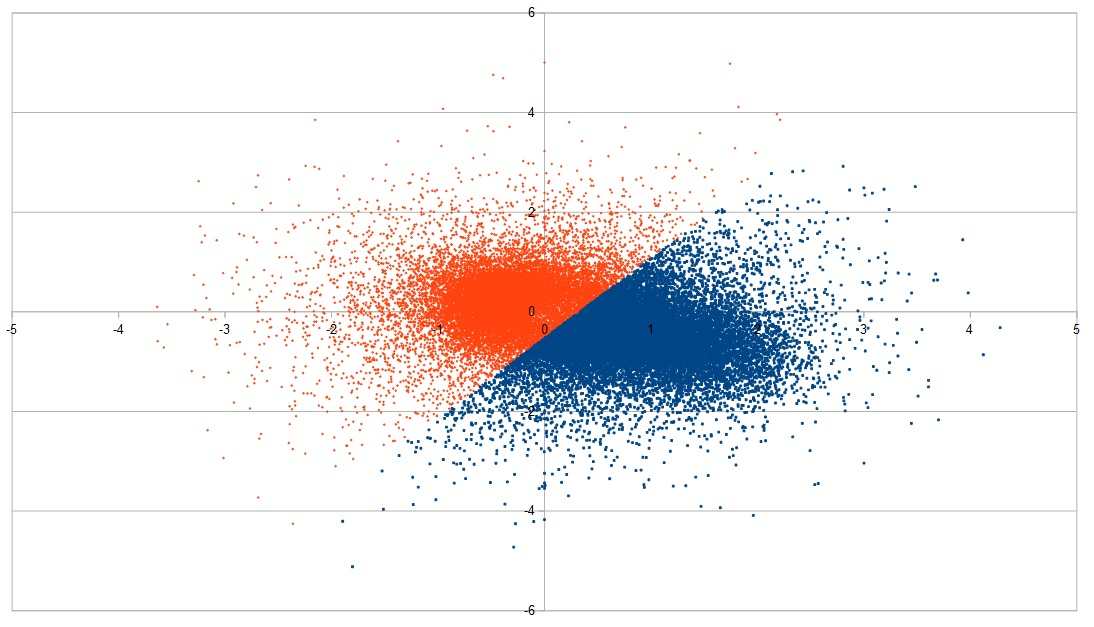
\includegraphics[scale=0.5]{Figures/kmeans_results}}
\par\end{centering}

\textcolor{black}{\protect\caption{\label{fig:Results-of-K-Means}Results of K-Means clustering algorithm
with $K=2$., on the edge gradients detected using Canny, from Kalahari.
The blue cluster represents the dune crestline gradients, and the
red represents all other non-crestline edges. The cluster centers
of blue is (0.8958, -0.5496), and the cluster center of the red is
(-0.4111, 0.2705).}
}

\end{figure*}


\textcolor{black}{The centroid values for each cluster are displayed
in \ref{fig:Results-of-K-Means}, which clearly indicates that the
blue cluster contains the stronger edges, which are more than likely
crestlines. To prove this, figure \ref{fig:Results-of-filtering}a.
shows the results of rejecting all weaker cluster gradients, and keeping
the dominant cluster gradients.}

\textcolor{black}{}
\begin{figure}
\begin{centering}
\textcolor{black}{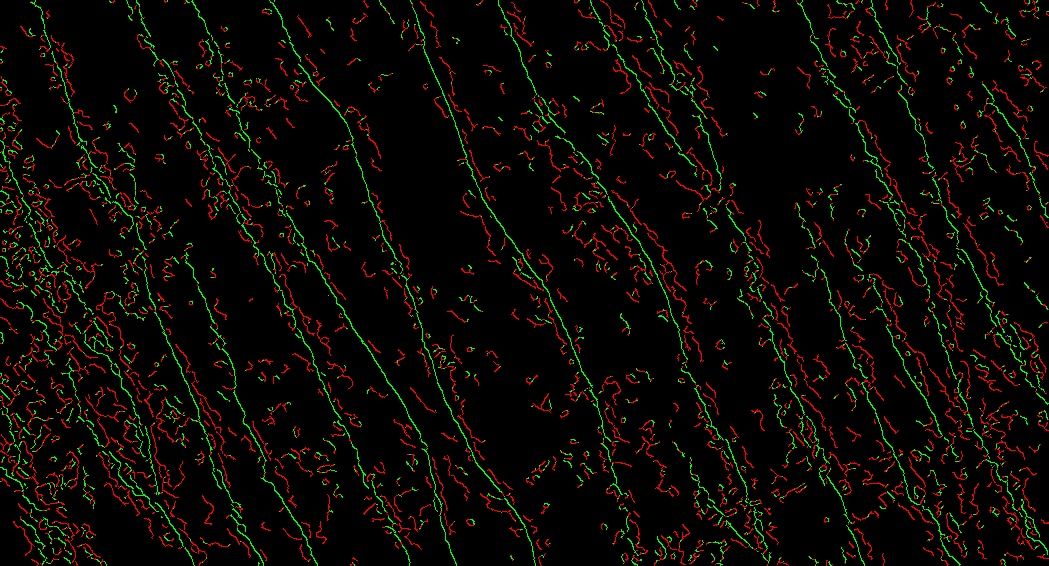
\includegraphics[scale=0.2]{Figures/filteredResults}}
\par\end{centering}

\begin{centering}
\textcolor{black}{(a)}
\par\end{centering}

\begin{centering}
\textcolor{black}{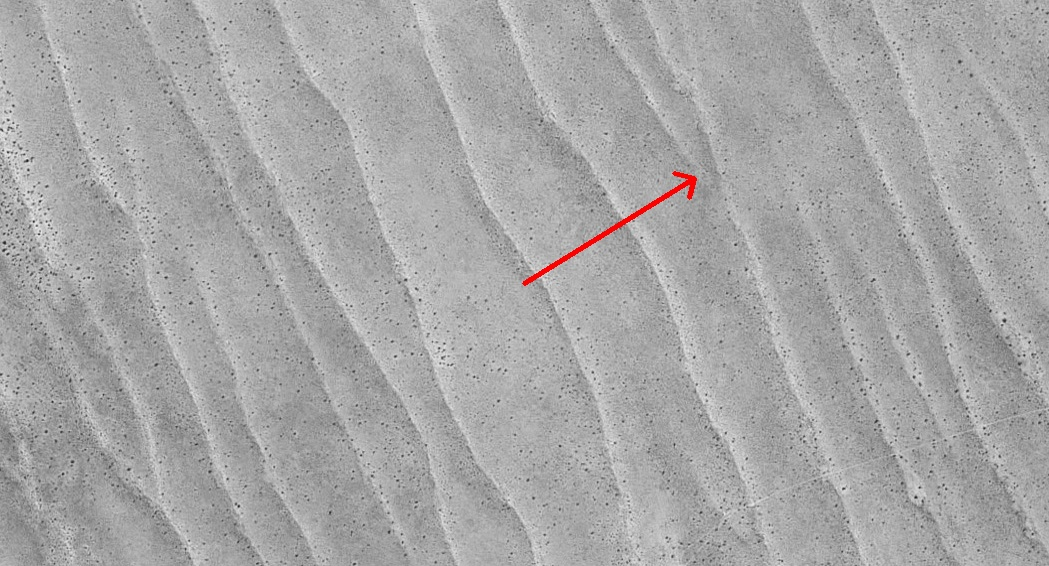
\includegraphics[scale=0.2]{Figures/orientationImg}}
\par\end{centering}

\begin{centering}
\textcolor{black}{(b)}
\par\end{centering}

\textcolor{black}{\protect\caption{\label{fig:Results-of-filtering}(a) Results of filtering out edges
(red) which belong to the cluster with the weaker edges. Potential
crestline edges (green) are preserved for use. (b) Average orientation
of the dominant cluster, which correctly appears to be perpendicular
to the trend of the crestlines.}
}
\end{figure}


\textcolor{black}{Once the weak edges have been filtered out, the
remaining edges are used as crestline candidates. The K-Means cluster
removes a majority of false positives, but does preserve some small
edge segments which are most likely noise. By using connected components
technique, these smaller less significant edge segments can be removed,
keeping only longer contiguous segments}\footnote{\textcolor{black}{More research can be done here. There may be techniques
used to fuse smaller segments into larger ones to achieve higher detection
accuracy}}\textcolor{black}{.}

\textcolor{black}{Results of this processing is displayed in section
\ref{sec:Results}.}


\paragraph*{\textcolor{black}{\uline{Using Histograms of Gradients}}\textcolor{black}{:}}

\textcolor{black}{An alternative to the clustering method is to compute
a histogram of the gradients based on orientation (REFERENCE NEEDED!!!).
Quantizing the space allows us to split edges according to their orientation,
where each bin in the histogram represents an edge orientation. Each
bin then covers an angle of $\frac{2\pi}{N}$radians, where }\textcolor{black}{\emph{N}}\textcolor{black}{{}
is the number of bins. }

\textcolor{black}{Each bin of the histogram is weighed by the magnitude
of edges. Once the histogram is constructed, peaks in the magnitude
will help determine the dominant orientation ($\varPhi$) of the dune
crestlines. The approach poses two main problems:}
\begin{enumerate}
\item \textcolor{black}{Determining }\textcolor{black}{\emph{N}}\textcolor{black}{:
In practice, a larger value for }\textcolor{black}{\emph{N}}\textcolor{black}{{}
has shown to provide finer grain resolution which improves dominant
orientation determination. In Figure \ref{fig:Resuls-of-unnormalized}
a value of $N=18$ is used}\footnote{\textcolor{black}{The optimal value for }\textcolor{black}{\emph{N}}\textcolor{black}{{}
has not yet been determined, but at first glance, smaller values for
}\textcolor{black}{\emph{N}}\textcolor{black}{{} will cause issues,
while larger values seem to improve results.}}
\item \textcolor{black}{Multiple Peaks: Often, images may have multple peaks
in the histogram, but only one of the peaks should represents the
true dominant orientation of crestlines.}
\end{enumerate}
\textcolor{black}{One assumption made is that the bin with the largest
value represents the orientation of the crestline edges. Although
this assumption holds for many cases, it is not always the case. The
Skeleton Coast test image provides a good example of this case in
Figure \ref{fig:Resuls-of-unnormalized}. In this particular case,
the are two major peaks in the histogram, where the stronger is not
the part of the crestline edge group, and the weaker one is.}

\textcolor{black}{Choosing the higher peak will cause invalid crestlines
to be chosen. In order to determine which peak best represents the
crestline edge group, some normalization can be applied. The normalization
process begins by computing the mean vector of the gradients from
the edge image as follows:}

\textcolor{black}{
\[
\hat{\mu}\left\langle \bar{x},\bar{y}\right\rangle =\left\langle \frac{\sum_{i=0}^{P}\delta_{x_{i}}}{P},\frac{\sum_{i=0}^{P}\delta_{y_{i}}}{P}\right\rangle 
\]
}

\textcolor{black}{where }\textcolor{black}{\emph{P}}\textcolor{black}{{}
is the total number of detected edges from the Canny edge detector,
$\delta_{x_{i}}$ and $\delta_{y_{i}}$ are the }\textcolor{black}{\emph{x}}\textcolor{black}{{}
and }\textcolor{black}{\emph{y}}\textcolor{black}{{} gradient component
of the }\textcolor{black}{\emph{i}}\textcolor{black}{th point. The
mean orientation is computed from the mean vector as:}

\textcolor{black}{
\[
\bar{\theta_{\mu}}=\arctan\left(\frac{\mu_{\bar{y}}}{\mu_{\bar{x}}}\right)
\]
}

\textcolor{black}{The gradients are then normalized by simply subtracting
the mean vector from each gradient:}

\textcolor{black}{
\[
\dot{\delta}\left(x_{i},y_{i}\right)=\left(\delta_{x_{i}}-\mu_{\bar{x}},\delta_{y_{i}}-\mu_{\bar{y}}\right)
\]
}

\textcolor{black}{The normalized orientation $\dot{\theta_{i}}$ can
then be computed:}

\textcolor{black}{
\[
\dot{\theta_{i}}=\arctan\left(\frac{\dot{\delta_{y_{i}}}}{\dot{\delta_{x_{i}}}}\right)-\bar{\theta_{\mu}}
\]
}

\textcolor{black}{To determine which bin the }\textcolor{black}{\emph{i}}\textcolor{black}{th
edge point belongs to, we simply calculate $\left\lceil \frac{\dot{\theta_{i}}\centerdot N}{2\pi}-0.5\right\rceil $,
and increment that bin by the magnitude of the normalized gradient
by $\sqrt{\dot{\delta}_{x_{i}}^{2}+\dot{\delta}_{y_{i}}^{2}}$. In
essense, this normalization process removes the uneven skew of the
gradients in the overall image. Removing this skew allows true crestline
edges to be fairly compared with other stronger edges. As shown in
Figure \ref{fig:Resuls-of-unnormalized}, the normalization process
softens the stronger dominant edge and enhances the true crestline
edges. This process enables crestlines to be accurately detected in
images where the valleys of dunes are sharp and contain strong edges}\footnote{\textcolor{black}{The gradient normalization process has not be proven
to work for all cases, only for the images from the test set. There
may be cases where the normalization may have the opposite effect
and remove all true crestline. More investigation and sample images
are required to determine the effectiveness of the normalization.}}\textcolor{black}{.}

\textcolor{black}{}
\begin{figure}
\begin{centering}
\textcolor{black}{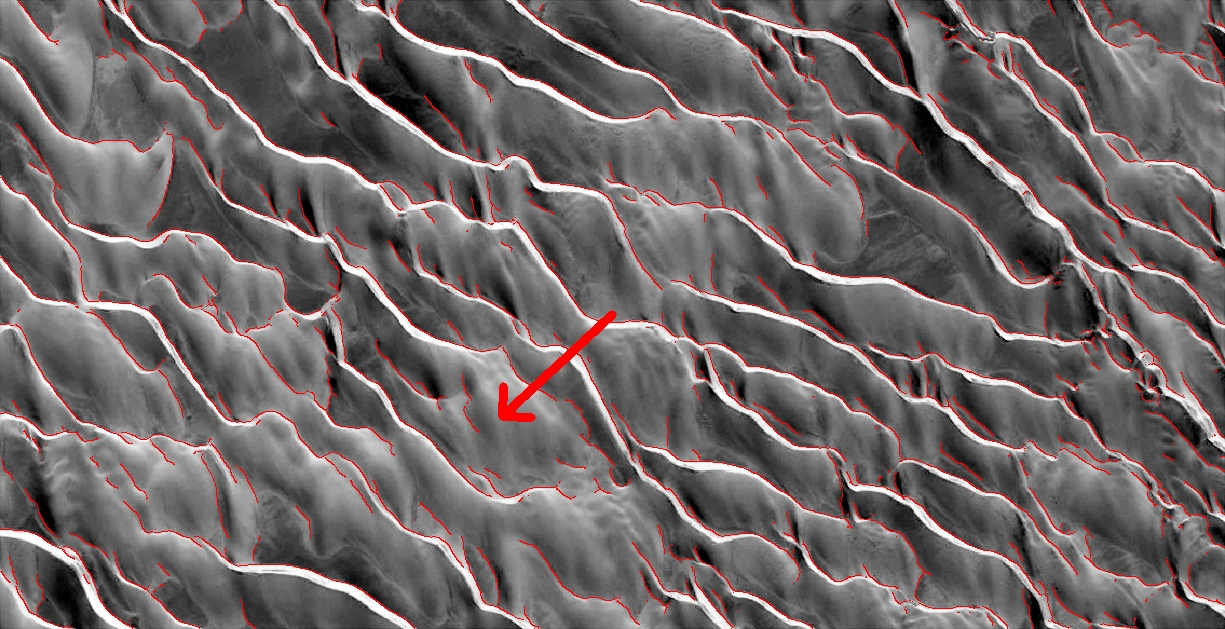
\includegraphics[scale=0.2]{Figures/hog_unnorm_results}}
\par\end{centering}

\begin{centering}
\textcolor{black}{(a)}
\par\end{centering}

\begin{centering}
\textcolor{black}{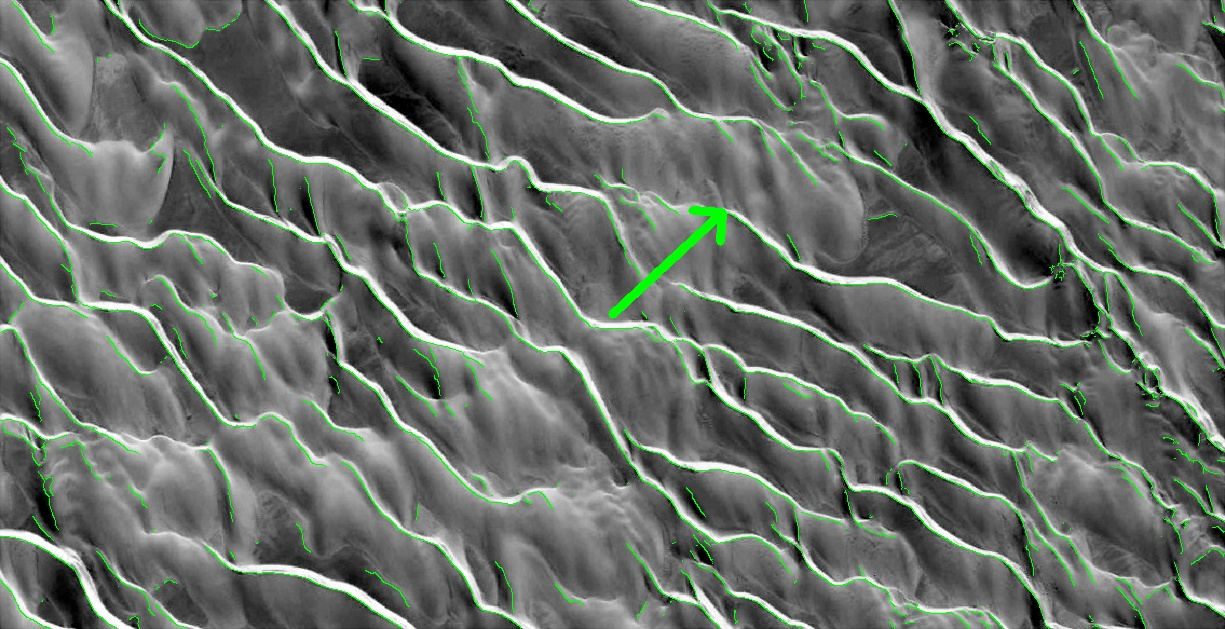
\includegraphics[scale=0.2]{Figures/hog_norm_results}}
\par\end{centering}

\begin{centering}
\textcolor{black}{(b)}
\par\end{centering}

\begin{centering}
\textcolor{black}{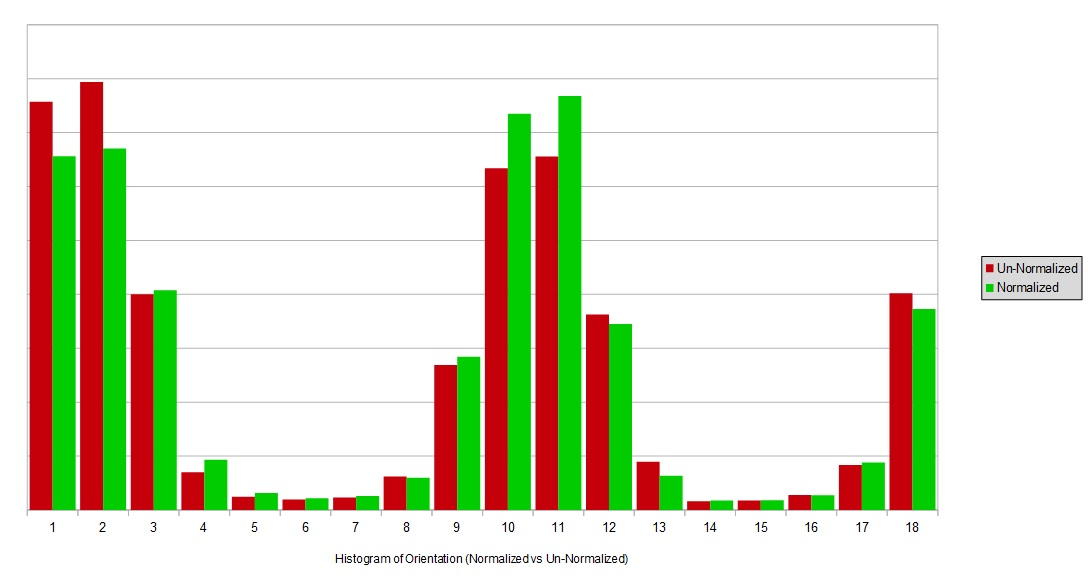
\includegraphics[scale=0.35]{Figures/hog_unnorm_histogram}}
\par\end{centering}

\begin{centering}
\textcolor{black}{(c)}
\par\end{centering}

\begin{centering}

\par\end{centering}

\textcolor{black}{\protect\caption{\textcolor{black}{\label{fig:Resuls-of-unnormalized}Results of unnormalized
(red) and normalized (green) histograms of gradients ($N=18$). The
histogram contains two major peaks, but the crestline is the weaker
of the two peaks. (a) Edges which belong to the dominant orientation
whic are invalid crestlines. (b) With normalization, the true crestlines
now have the higher overall magnitude. (c) The 18 bin histogram of
gradients witth and without normalization.}}
}
\end{figure}


\textcolor{black}{The dominant orientation can be used to filter out
most non-crestline edges by keeping all edges using the following
criteria:}

\textcolor{black}{
\begin{equation}
P\left(x_{i},y_{i}\right)=\begin{cases}
1 & \left\Vert \arctan\left(\frac{\delta_{y_{i}}}{\delta_{x_{i}}}\right)-\varPhi\right\Vert \leqq\varphi\\
0 & otherwise
\end{cases}\label{eq:edge-criteria}
\end{equation}
}

\textcolor{black}{\emph{P}}\textcolor{black}{{} is a crestline candidate
if it satisfies the orientation criteria, where $\varphi$ is an angle
tolerance value which is experimentally set to $\varphi=\frac{\pi}{2}$}\footnote{\textcolor{black}{The value of $\varphi$ has not been extensively
tested yet, and may have an effect on the results, more testing is
required to determine the sensitivity of this parameter.}}\textcolor{black}{{} .}

\textcolor{black}{\sout{In order to improve the robustness, a connected
components method is used to find all segments from the canny image.
For each segments if the number of points along the segment satisfy
the criteria from \mbox{\ref{eq:edge-criteria}} is greater than some
ratio R, then the segment is considered to be a dune segment, where
$0<R<1$. Choosing a small R generally improves the true positive
detection, while increasing false positive rate}}\footnote{\textcolor{black}{\sout{During initial testing, R (\textasciitilde{}0.1)
was set to a very low value, which allowed many of the true positive
to be found at the expense of a higher false positive rate. This technique
is very simplistic and does require more investigation to improve
on.}}}\textcolor{black}{\sout{.}}


\subsubsection*{\textcolor{black}{Dune segment linking}}

\textcolor{black}{With the dominant orientation computed, many false
positives have been rejected. The next step of the process is to group
segments which link together. Since each crestline candidate segments
is a collections of two dimensional points, an intuitive step is to
fit a line to the candidate segments. The line fitting algorithm used
is from the OpenCV library \cite{opencv_library}, which aims to minimize:}

\textcolor{black}{
\[
\sum_{i}\rho\left(r_{i}\right)
\]
}

\textcolor{black}{where $r_{i}$ is the distance between a point an
the line, and $\rho\left(r_{i}\right)$ is the function used. We use
the simplest least square method,$\rho\left(r\right)=\frac{r^{2}}{2}$.
The result of the line fitting produces a vector of four values $\left\langle x,y,v_{x},v_{y}\right\rangle $,
where the (}\textcolor{black}{\emph{x}}\textcolor{black}{, }\textcolor{black}{\emph{y}}\textcolor{black}{)}\textcolor{black}{\emph{
}}\textcolor{black}{components are the position of the line, and $(v_{x},v_{y})$
is the normalized vector which is colinear to the line, encoding the
orientation of the line.}

\textcolor{black}{With all segments fit with a line, we can filter
the segments based on the orientations of the lines. To get a general
view of the distribution of the orientation of the lines, a histogram
of the line orientations can help determine dominant lines. The histogram
can be constructed based on the orientation of the lines, weighed
by segment length. As shown in figure \ref{fig:Results-of-filtering-1}(a),
the histogram appears to have a unimodal distribution. When choosing
all lines which belong to the peak bin in the histogram, the resulting
in the output image \ref{fig:Results-of-filtering-1}(b). The results
show that many of the false positives have been filtered out.}

\textcolor{black}{Since the shown distribution appears to be unimodal,
a better approach may be to simply compute the mean and standard deviation
of the line orientations. Choosing the appropriate sigma value to
filter out the noise and false positives depends on the distribution.
In some cases, such as images with crestlines which are more curved,
the variation orientations may be more significant.}

\textcolor{black}{}
\begin{figure}
\begin{centering}
\textcolor{black}{(a) 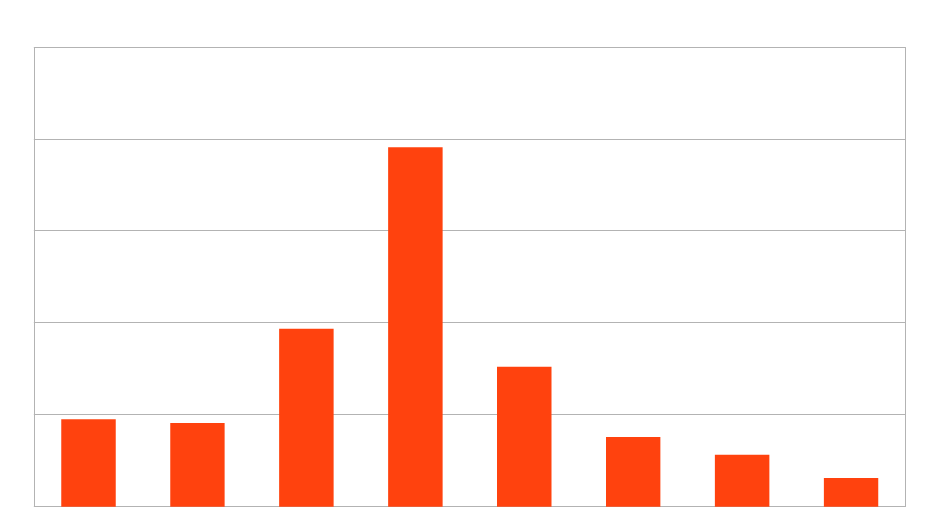
\includegraphics[scale=0.2]{Figures/linehistogram1}}
\par\end{centering}

\begin{centering}
\textcolor{black}{(b) 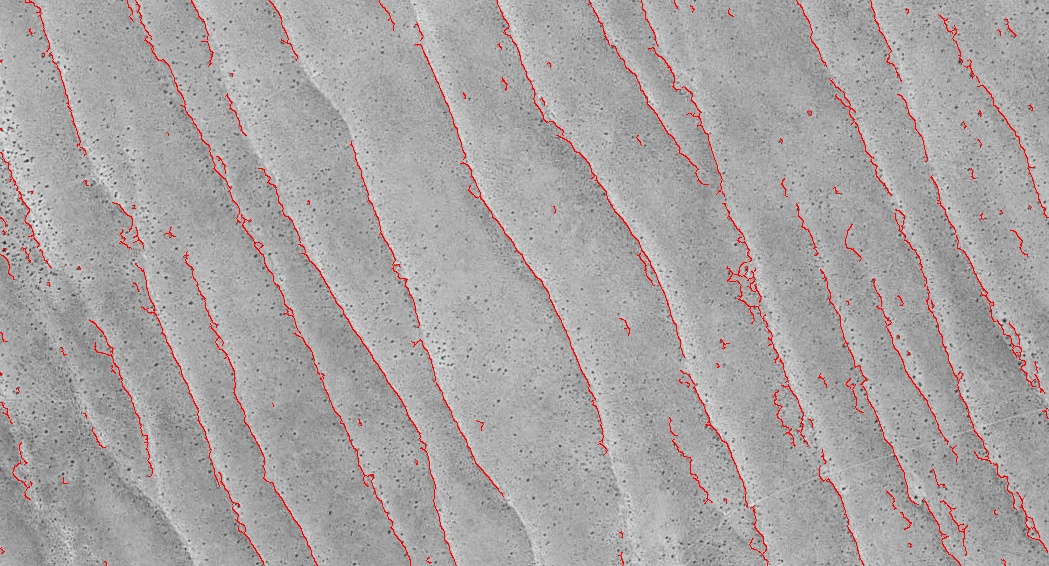
\includegraphics[scale=0.22]{Figures/FilteredFitLines}}
\par\end{centering}

\begin{centering}
\textcolor{black}{(c) 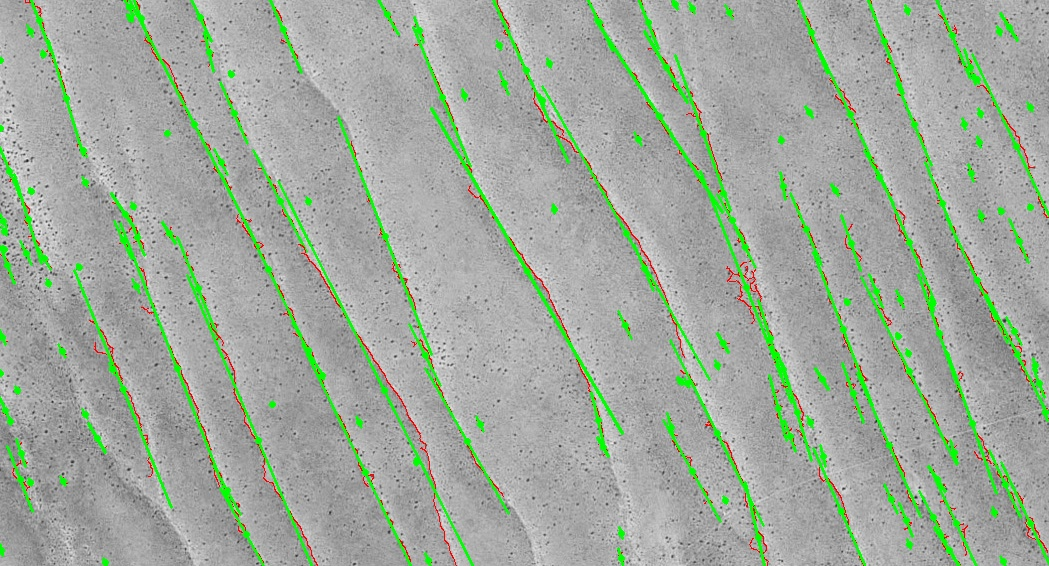
\includegraphics[scale=0.22]{Figures/FilteredFitLines_lines}}
\par\end{centering}

\textcolor{black}{\protect\caption{\textcolor{black}{\label{fig:Results-of-filtering-1}Results of filtering
based on the line orientation fitting, and choosing the peak in the
histogram. (a) the histogram of line orientations weighed by segment
lenght, (b) segments which have orientation matching the peak in the
histogram, (c) the fitted lines from the dune segments.}}
}
\end{figure}


\textcolor{black}{In order to avoid the filtering of true positives,
a linking algorithm should be used to link segments which belong to
the same crest-line.}


\subsubsection{\textcolor{black}{Method \#3: Watershed Segmentation}}

\textcolor{black}{In an approach similar to \ref{sub:Method-=0000231:-Adaptive},
the goal of this approach is to segment out the brighter region of
the image, which represents the sunny side of the dune, using the
watershed transform. This powerful segmentation tool is used to determine
the boundary of the bright dune region, better than a simple thresholding
method.}

\textcolor{black}{In order to extract reliable regions, image illumination
normalization is applied, to make the illumination more evenly distributed
accross an image. After applying some pre-processing to the image
(Median and Gaussian blurring to remove as much noise as possible),
the illumination normalization}\footnote{\textcolor{black}{The illumination normalization presented is very
basic, and better normalization schemes should be tried.}}\textcolor{black}{{} is applied to the image as shown in Figure \ref{fig:Illumination-Normalization-using}.}

\textcolor{black}{The normalization process is done in a fairly simple
and efficient way, using integral images. The integral images was
orignially proposed in \cite{Summed-area-tables-for-texture-mapping},
and was popularized for computer vision applications by \cite{Robust-real-time-Object-Detection}.
The integral image representation allows rectangular features to be
computed very efficiently. Each pixel (x,y) of the integral image
is the sum of the pixels above and to the left of it, as described
in \cite{Robust-real-time-Object-Detection}:}

\textcolor{black}{
\[
ii\left(x,y\right)=\sum_{x'\leq x,y'\leq y}i\left(x',y'\right)
\]
}

\textcolor{black}{To normalize using integral images, the mean $\mu_{i}$
of the image, which can be done efficiently once the integral images
is computed, given an $N\times M$ image.}

\textcolor{black}{
\[
\mu_{i}=\frac{ii\left(M,N\right)}{M\cdot N}
\]
}

\textcolor{black}{The goal of the illumination normalization is to
bring pixel intensities value closer to the mean intensity of the
image for a more even distribution of intensities. To accomplish this
we simply compute a ratio multiplier of the mean intensity $\mu_{i}$
over the square local area ($w\times w$ ) mean intensity centered
around a pixel (x,y). The mean of a local area can be computed efficiently
using the integral image theory:}

\textcolor{black}{
\[
\mu_{l}\left(x,y\right)=D-C-B+A
\]
}

\textcolor{black}{
\[
A=ii\left(x-\frac{w}{2},y-\frac{w}{2}\right)
\]
}

\textcolor{black}{
\[
B=ii\left(x+\frac{w}{2},y-\frac{w}{2}\right)
\]
}

\textcolor{black}{
\[
C=ii\left(x-\frac{w}{2},y+\frac{w}{2}\right)
\]
}

\textcolor{black}{
\[
D=ii\left(x+\frac{w}{2},y+\frac{w}{2}\right)
\]
}

\textcolor{black}{Then, the ratio of image intensity to local mean
intensity simply is $r_{\mu_{l}\left(x,y\right)}=\frac{\mu_{i}}{\mu_{l}\left(x,y\right)}$.
The pixel intensity value at that location is then multipled by this
ratio to get the normalized value:}

\textcolor{black}{
\[
\tilde{i}\left(x,y\right)=r_{\mu_{l}\left(x,y\right)}\cdot i\left(x,y\right)
\]
}

\textcolor{black}{}
\begin{figure}
\begin{centering}
\textcolor{black}{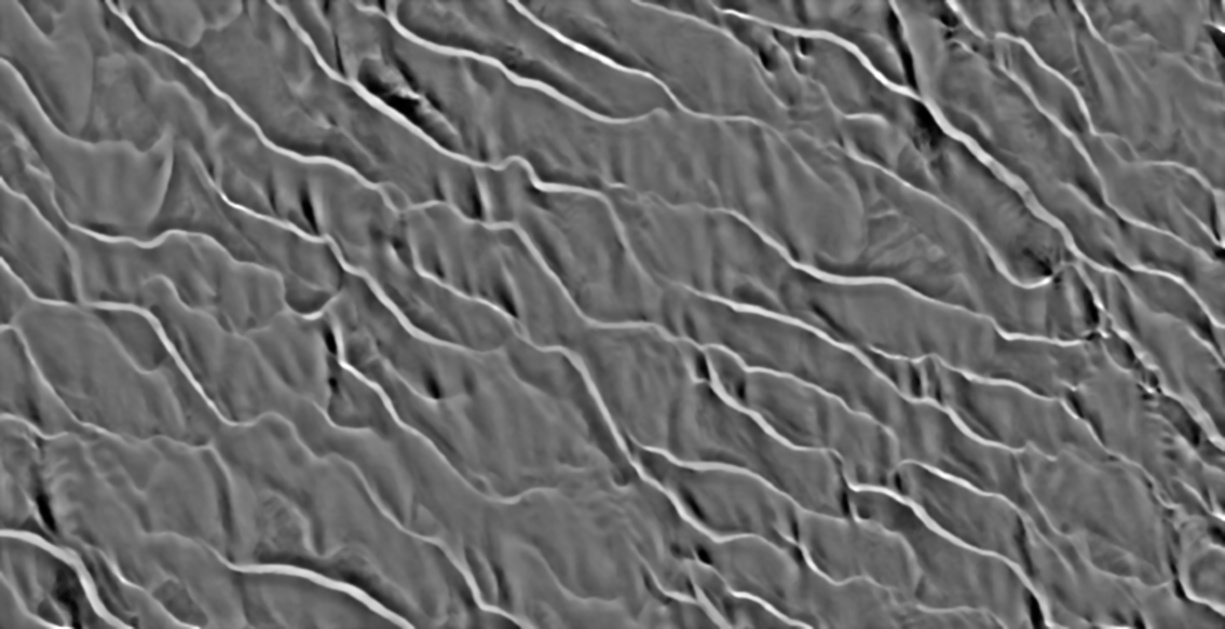
\includegraphics[scale=0.2]{Figures/normalizedIllumination}}
\par\end{centering}

\textcolor{black}{\protect\caption{\textcolor{red}{\label{fig:Illumination-Normalization-using}Illumination
Normalization using integral images with }\textcolor{red}{\emph{w}}\textcolor{red}{{}
= 30 }}
}
\end{figure}


\textcolor{black}{With the image illumation normalized, the watershed
transform can be used to segment out the brighter regions of the image
which will be the dune sunny sides. The watershed implementation used
is provided by the OpenCV library, and is a variant of the implementation
proposed in \cite{Color-image-segmentation}. The watershed uses an
initial seed rough image of the desired locations to segment out,
which in this application is the brighter regions of the image.}

\textcolor{black}{The desired regions to extract are the bright and
shaded areas. The threshold values for these can be determined from
the image's mean and standard deviation intensity values:}

\textcolor{black}{
\[
T_{high}=\mu_{i}+\rho_{high}\cdot\sigma_{i}
\]
}

\textcolor{black}{
\[
T_{low}=\mu_{i}+\rho_{low}\cdot\sigma_{i}
\]
}

\textcolor{black}{Where the $\rho_{high}$ and $\rho_{low}$ are scalar
values determined empirically. All pixels above the high threshold
are labeled as the desired region to segment (in white), and all pixels
below the lower threshold are set to the non-desired region (in gray).
A morphological eroding operation is applied to better seperate the
regions for the watershed transform. Using the labeled image and normalized
illumination image, the watershed algorithm is able to segment out
the dune regions reliably, as shown in Figure .}

\textcolor{black}{}
\begin{figure}
\begin{centering}
\textcolor{black}{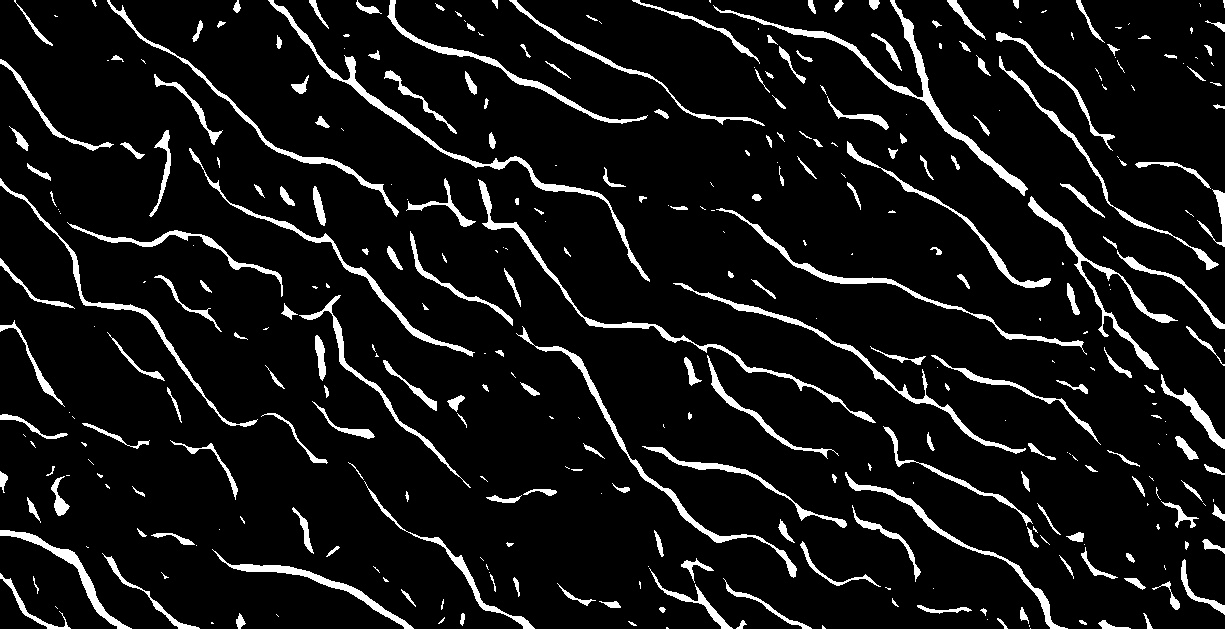
\includegraphics[scale=0.2]{Figures/sunnylabel}}
\par\end{centering}

\begin{centering}
\textcolor{black}{(a)}
\par\end{centering}

\begin{centering}
\textcolor{black}{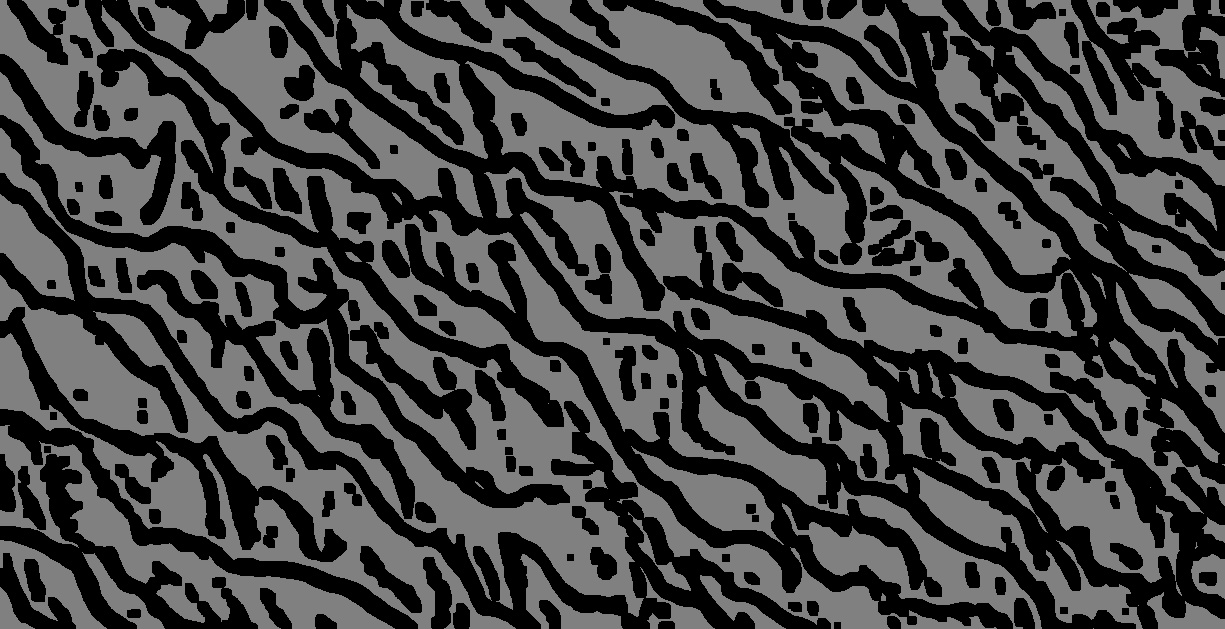
\includegraphics[scale=0.2]{Figures/shadedlabel}}
\par\end{centering}

\begin{centering}
\textcolor{black}{(b)}
\par\end{centering}

\begin{centering}
\textcolor{black}{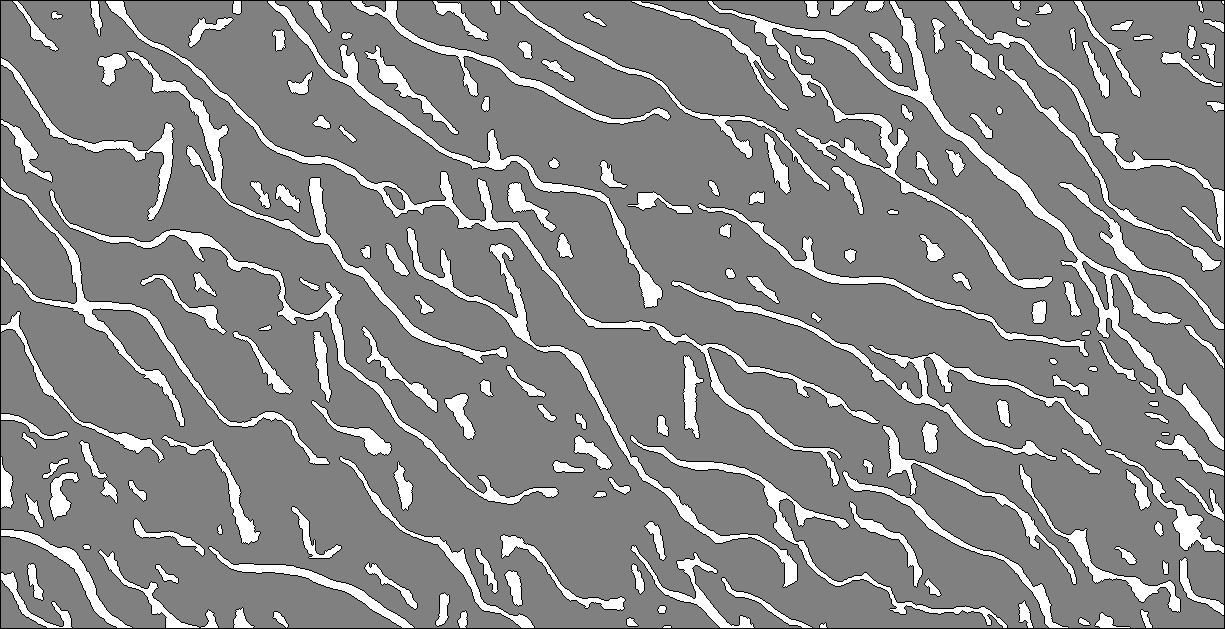
\includegraphics[scale=0.2]{Figures/watershedResultingMarkers}}
\par\end{centering}

\begin{centering}
\textcolor{black}{(c)}
\par\end{centering}

\textcolor{black}{\protect\caption{\textcolor{red}{\label{fig:Watershed-segmentation-process}Watershed
segmentation process with $\rho_{high}=0.8$ and $\rho_{low}=0.4$,
(a) Result of the high threshold, (b) Result of low threshold, (c)
Watershed segmentation results}}
}
\end{figure}


\textcolor{black}{After computing the watershed segmentation image,
the regions extracted from it can be retrieved using contour detection,
as done in section \ref{sub:Method-=0000231:-Adaptive}. }

\textcolor{black}{The contours retrieved are closed loops where one
segment will be along the dune crest line and the other not. To determine
which segments of the coutour belong to the dune crestline, we can
use what was learned from section \ref{sub:Method-=0000232:-Unsupervized}.
Building a histogram of the image gradients, choosing the dominant
orientation, and filtering out all contour points which do not agree
with the dominant orientation. }

\textcolor{black}{The results of the filtering are shown in Figure
\ref{fig:Dune-Crestline-detection}, and the accuracy of these results
are shown in Table \ref{tab:Results-of-the}. There are a few drawbacks
so far:}
\begin{enumerate}
\item \textcolor{black}{An assumption that a dune contains a bright side.
Not all images (especially the Simpson image), have crestlines that
have a bright edge.}
\item \textcolor{black}{The edges of the contours appear to be slightly
noisier than edge-based approaches.}
\item \textcolor{black}{Localization of the segments is poor. Some segments
do not lie on an actual edge, which may be reported as a false positive.}
\end{enumerate}
\textcolor{black}{On the other hand, the watershed approach appears
to have some benefits:}
\begin{enumerate}
\item \textcolor{black}{Better connectivity of dune crestline segments.
When edges become weak between two connecting segments, the edge based
approaches produce gaps, where the watershed is able to fill the gaps.}
\item \textcolor{black}{Watershed method could be further expanded to include
color image processing.}
\end{enumerate}

\subsubsection{\textcolor{black}{Method \#4: Frequency Domain}}

\textcolor{black}{In this approach, we take advantage of the fact
dune-field patterns seem to to have some periodic pattern, which could
possibly be extracted from the frequency domain. Converting the images
into the frequency domain using the Discrete Fourier Transform (DFT)
(REFERENCE NEEDED) provides a method for applying some processing
on individual frequencies of the image.}


\paragraph*{\textcolor{black}{\uline{Feature extraction from the frequency
domain}}\textcolor{black}{:}}

\textcolor{black}{In this application, the features we desire to extract
are the dune crest-lines, which in the spacial domain are edges. In
the frequency domain, the crest-lines may belong to some of the higher
frequencies (or possibly a subset of the frequency spectrum). The
shifted frequency domain output of the DFT is shown in Figure \ref{fig:Frequency-spectrum-results}.}

\textcolor{black}{From the frequency domain, dominant frequencies
can be extracted by searching for large magnitudes of frequencies
}\footnote{\textcolor{black}{Determining which frequencies to extract will be
key for this application. More research needs to be done on how to
extract features from the frequency domain.}}\textcolor{black}{. Typically, from the dataset used, it can be shown
that a dominant orientation in the frequency appears to be present
in the dune-field images. From preliminary observations, the dominant
orientation seems to correlate exactly which the orientation of the
dune crests.}

\textcolor{black}{In order to determine this dominant orientation,
the frequency domain magnitude image is thresholded based on the mean
and standard deviation of the frequency magnitudes, as shown in Figure
\ref{fig:Frequency-spectrum-results}. Because output of this threshold
is somewhat noisy, a median filter is applied to create a smooth region
of for the dominant frequency. The contour of the region is then extracted,
which is used to fit an ellipse.}

\textcolor{black}{The computed ellipse's orientation appears to match
the orientation of the dune gradients. The information provided by
the ellipse may prove useful }\footnote{\textcolor{black}{Fitting an ellipse is currently mainly used for
determining the orientation of the gradients of the dune crests. Since
I am not too familiar with the frequency domain, there may be a better
approach to extract this, or other features.}}\textcolor{black}{. Currently, we use this ellipse to generate the
mask for high-pass filtering. The mask shown in Figure\ref{fig:Frequency-spectrum-results}
simply rejects all lower frequencies (close to the center of the spectrum),
and allows all higher frequencies to pass through. The effect produces
a kind of edge detection filter, where lower values could potentially
be used to determine locate dune crests. At first glance, the results
appear to be promising.}

\textcolor{black}{}
\begin{figure*}
\begin{centering}
\textcolor{black}{(a)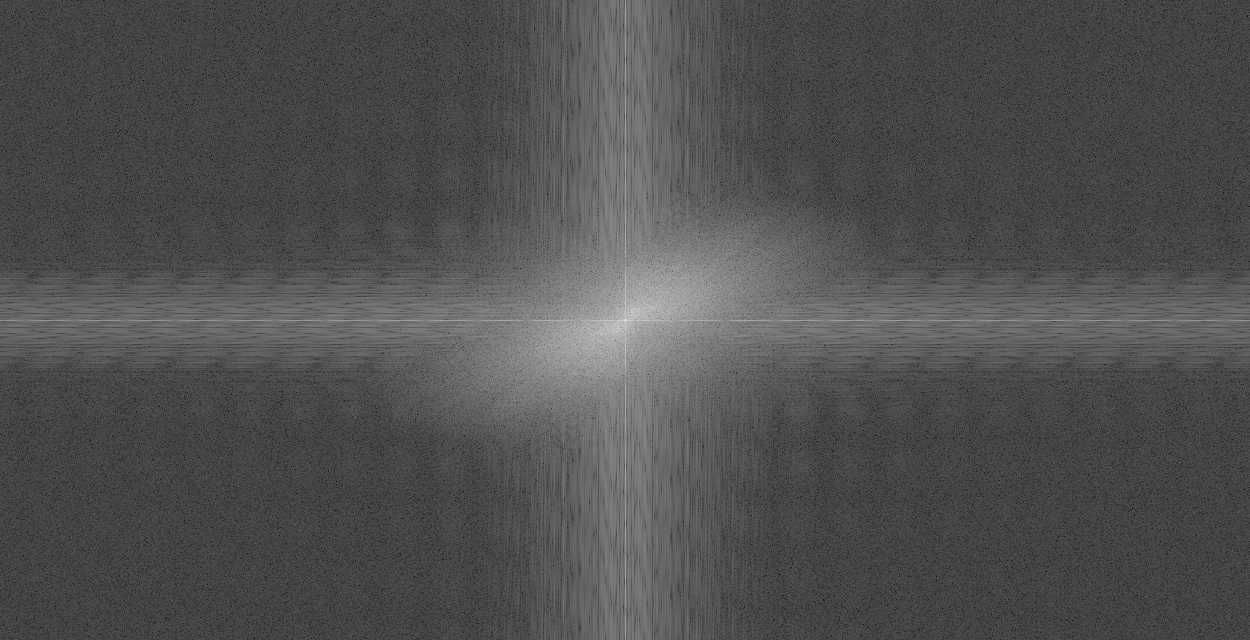
\includegraphics[scale=0.18]{Figures/DFT_spectrum}(b)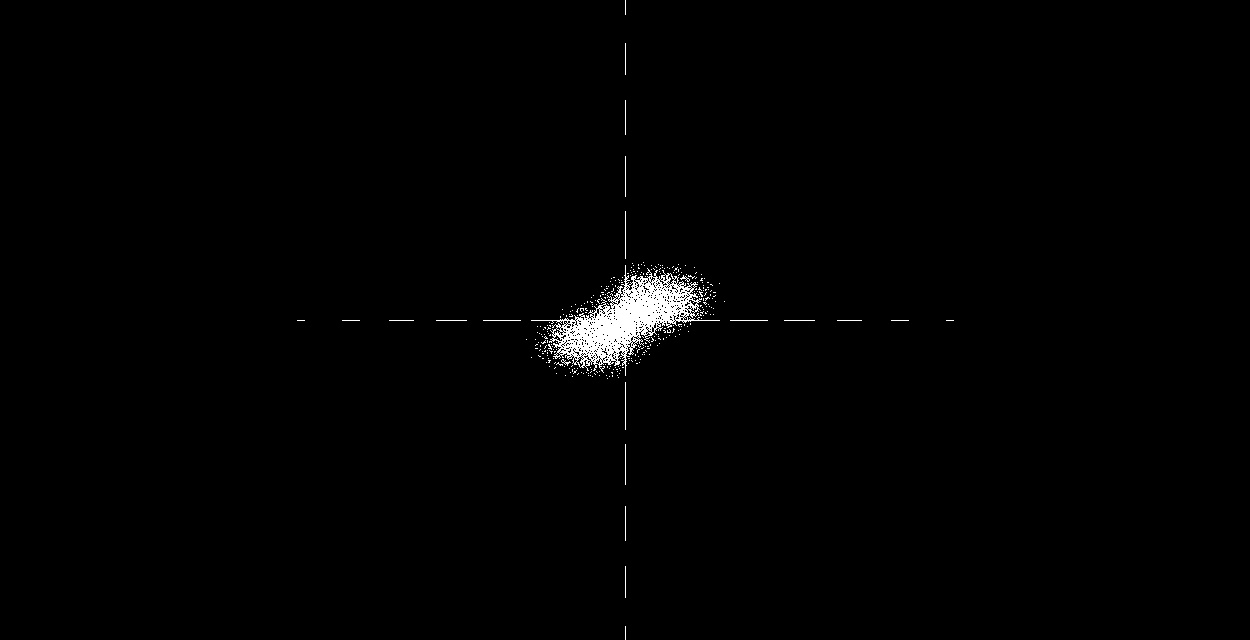
\includegraphics[scale=0.18]{Figures/DFT_spectrum_threshold}}
\par\end{centering}

\begin{centering}
\textcolor{black}{(c)
\includegraphics[scale=0.18]{Figures/DFT_spectrum_threshold_median}(d)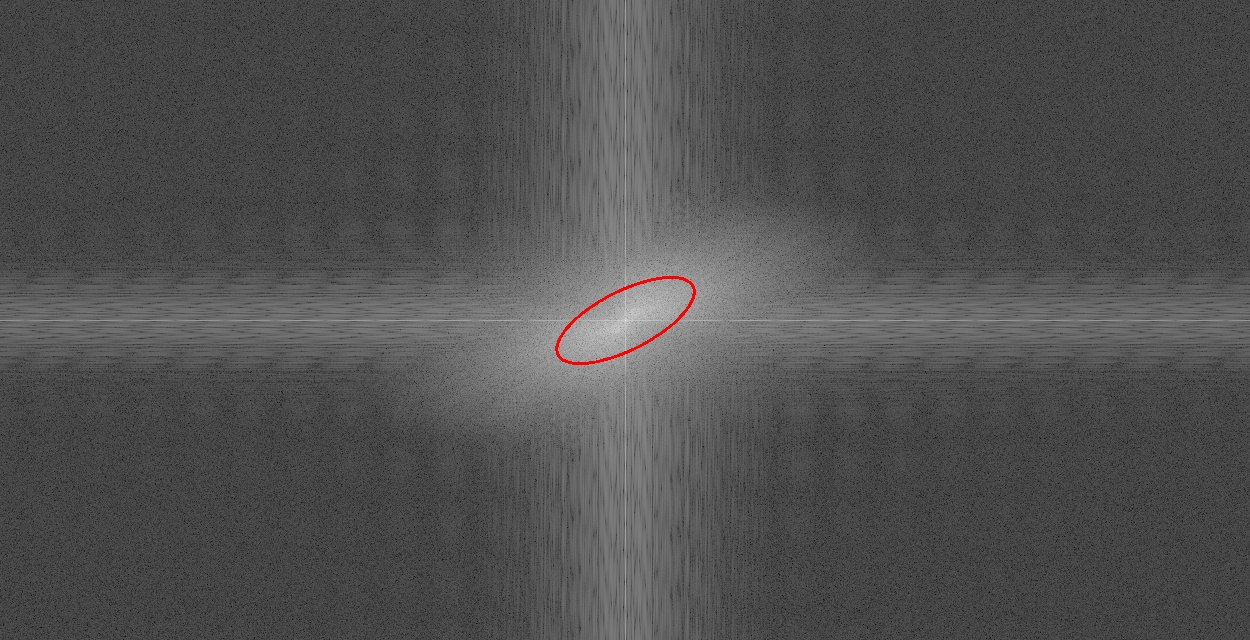
\includegraphics[scale=0.18]{Figures/DFT_spectrum_ellipsefit}}
\par\end{centering}

\begin{centering}
\textcolor{black}{(e)
\includegraphics[scale=0.18]{Figures/DFT_mask}(f)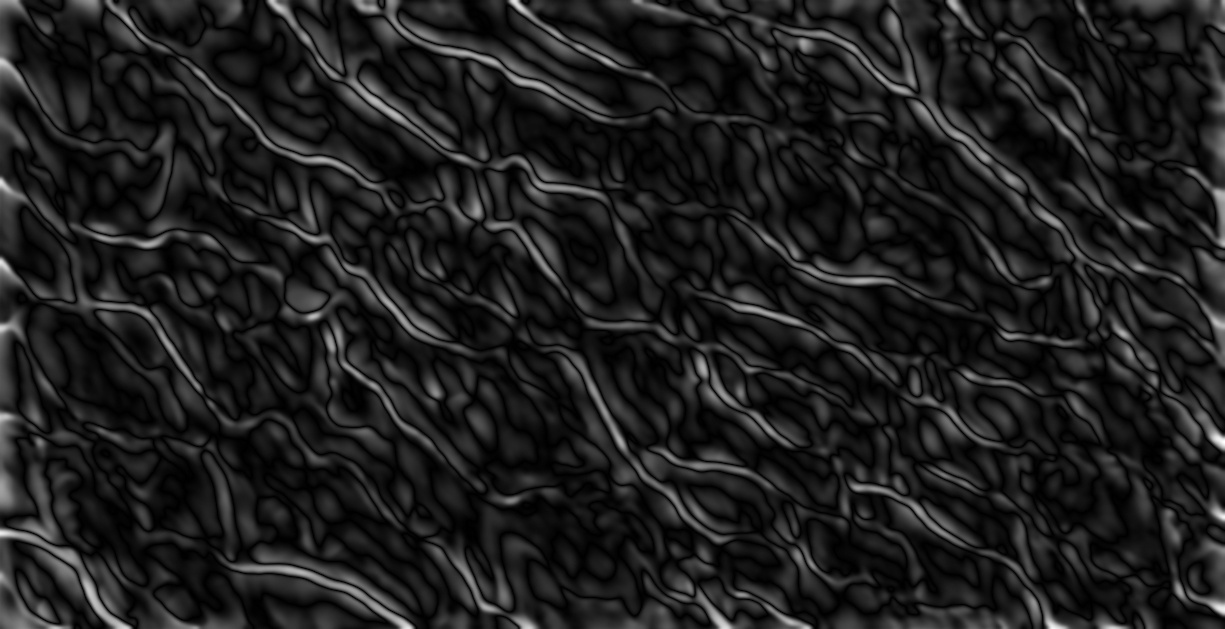
\includegraphics[scale=0.18]{Figures/DFT_HPF}}
\par\end{centering}

\textcolor{black}{\protect\caption{\textcolor{black}{\label{fig:Frequency-spectrum-results}Frequency
spectrum processing results from the Skeleton-Coast image. (a) Log-normalized
shifted frequency domain, (b) Result of thresholding frequency domain
magnitude based on average magnitude and standard deviation of the
magnitudes, (c) Median filtering of the binary image of the frequency
domain, (d) Result of ellipse fitting of the dominant frequencies
region, (e) Mask used for high-pass filtering of the frequency domain,
(f) Result inverse DFT of the high pass filter applied on the frequency
domain.}}
}
\end{figure*}



\subsubsection{\textcolor{black}{Method \#4: Edge Direction Based Approach}}

\textcolor{black}{In this approach, we used knowledge learned from
a previous edge based approach. In section \ref{sub:Method-=0000232:-Unsupervized},
we learning that the dominant orientation of the dune field could
be determined based on the derivative of the image. In that approach,
we used the gradient magnitudes to find major crest-line edges, and
filtered out edges which do not agree with the dominant orientation
of the gradients.}

\textcolor{black}{Using edges provides good localization but is prone
to discontinuity of edge segments. A better alternative explored is
to use the image of the gradient directions and find regions which
agree with the dominant orientation. The regions produces by the gradient
direction map have been shown to be typically smooth and have good
continuity in this application. }

\textcolor{black}{The main reason for this is the nature of the problem
itself, since dunes have a bright and shaded side. As gradients approach
the crest-line, their direction component point towards the crest
line. The shaded side of the dune can be seen as a color gradient
ranging from dark to bright as it approaches the crest-line. This
trend is plotted clearly in Figure \ref{fig:The-gradient-direction}.
Once this pattern is identified, it is simply a matter of thresholding
the gradient direction map to retrieve regions which have gradients
along the dominant orientation.}

\textcolor{black}{}
\begin{figure}
\begin{centering}
\textcolor{black}{(a)}
\par\end{centering}

\begin{centering}
\textcolor{black}{\includegraphics[scale=0.24]{\string"E:/Projects/Thesis/DuneDetection/DuneDataset/WDC 1/WDC_1_image\string".jpg}}
\par\end{centering}

\begin{centering}
\textcolor{black}{(b)}
\par\end{centering}

\begin{centering}
\textcolor{black}{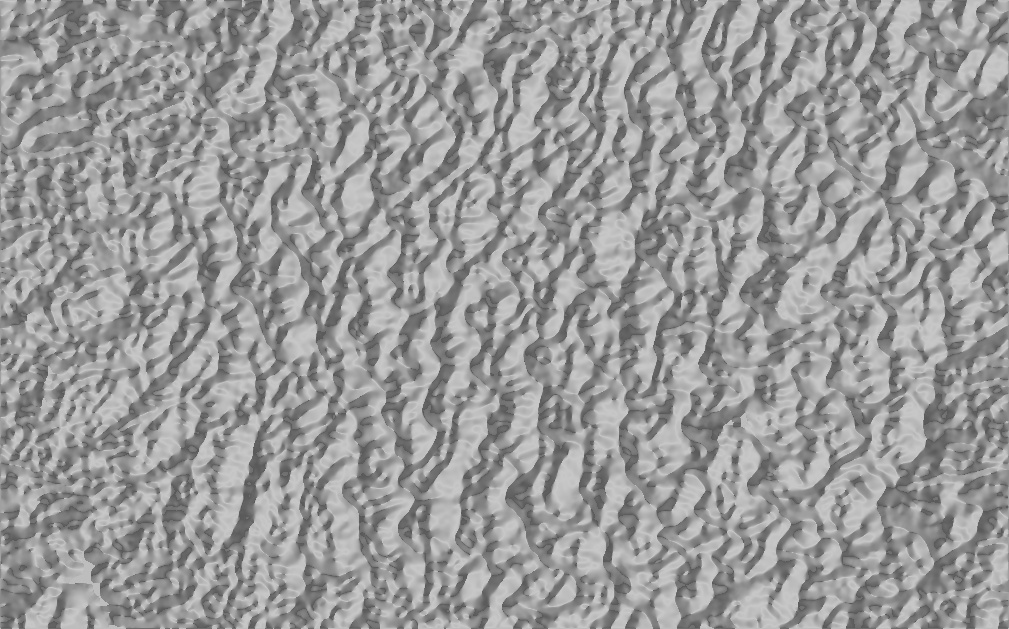
\includegraphics[scale=0.23]{Figures/NormalizedDirectionImage}}
\par\end{centering}

\begin{centering}
\textcolor{black}{(c)}
\par\end{centering}

\begin{centering}
\textcolor{black}{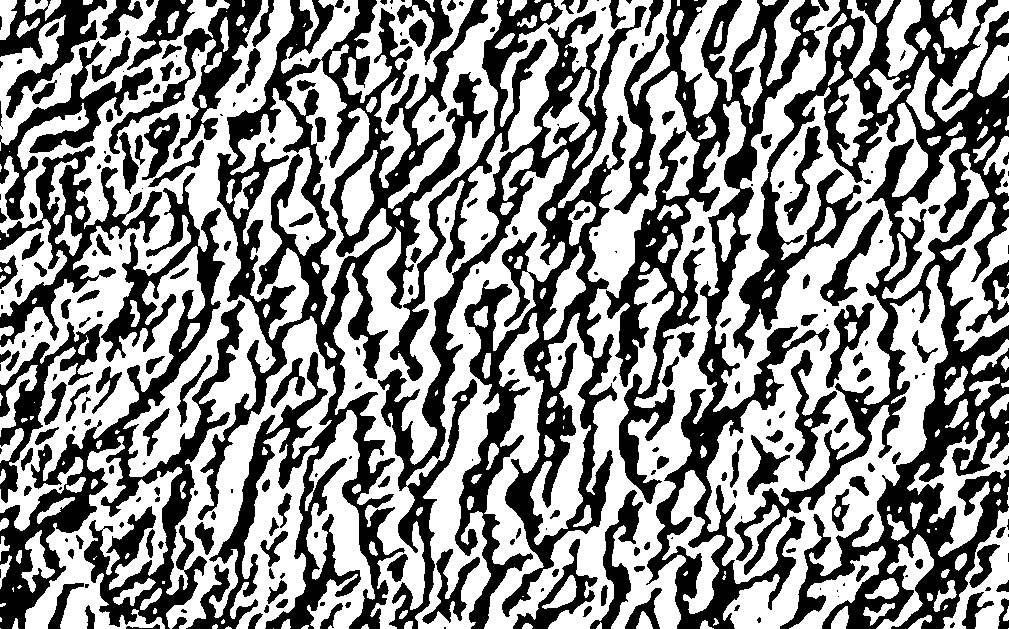
\includegraphics[scale=0.23]{Figures/ThresholdNormalizedDirectionImage}}
\par\end{centering}

\textcolor{black}{\protect\caption{\textcolor{black}{\label{fig:The-gradient-direction}The gradient
direction map based on the dominant orientation calculated for (a)
WDC image. (b) The normalized gradient direction based on the dominant
orientation. Brighter regions represent pixels which are along the
dominant orientation, while darker regions are gradients which oppose
the domination orientation. (c) The gradient direction map thresholded.
Pixels with $\left\Vert \theta_{i}-\theta_{dominant}\right\Vert \leq\frac{\pi}{2}$
are said to agree with the dominatn orientation, and set to white,
all others to 0.}}
}
\end{figure}


\textcolor{black}{Once the gradient direction map has been thresholded,
the binary image provides well defined regions which allows the use
of contours to determine the crest-lines. The contours extracted provide
good continuity of the crest-lines, but also contain many elements
which are not part of the crest-line. To reject segments of the contour
which are not part of the crestlines, three techniques have been tried.}


\paragraph{\textcolor{black}{1) Intensity Based:}}

\textcolor{black}{This algorithm uses intensity values of the pixels
along the contours. Segments of the contour which are on brighter
regions of the image are considered to be part of the crest-lines}\footnote{\textcolor{black}{The use of intensity values to determine which segments
of a contour are on the actual crest-line may not be an optimal solution,
but has provided adequate means of rejecting many false positives
for the time being.}}\textcolor{black}{.}

\textcolor{black}{The main benefit of this approach is that the resulting
regions have sharp and defined edges along the dune crest-line, regardless
of how sharp an edge is in actuality. In many cases, as is the case
in Figure \ref{fig:The-gradient-direction}, dunes in the same image
may have some sharp edges along the crest-line while others have less
defined crest-lines. Using gradient magnitude in areas with poorly
defined crest-lines yields poor results, while the gradient direction
maps provides a sharper edge and a better estimate of where a crest-line
may be. The downside of this method is that not using the gradient
magnitude results in poor localization of the actual crestline.}


\paragraph{\textcolor{black}{2) Gradient Based:}}

\textcolor{black}{This algorithm uses the gradient values of the pixels
along the contours.The gradient magnitudes provide much more accuracy
in localizing the desired crestlines. In order to improve localization,
the local gradient magnitude of the detected contours must be shifted
towards to nearest gradient magnitude peak. To accomplish this, a
search is applied from a candidate point on the contour in the opposite
direction of the dominant orientation. As shown in \ref{fig:Effect-of-K},
the parameter K will have a tendency to shift the contour lines towards
the dominant orientation. Therefore, searching in the opposite dirrection
of the dominant orientation for a peak in the gradient magnitude should
improve localization.}


\paragraph{\textcolor{black}{3) Intensity and Gradient:}}

\textcolor{black}{This algorithm uses a combination of the two methods
presented above. TODO: TRY THIS APPROACH!!!}


\paragraph{\textcolor{black}{Parameter Study}}

\textcolor{black}{For this approach, there are relatively few parameters
to optimize. The main parameters are:}
\begin{enumerate}
\item \textcolor{black}{The value of }\textcolor{black}{\emph{K}}\textcolor{black}{,
which determines the size of the kernel which computes the gradients.
The effects of varying this parameter are shown in Figure \ref{fig:Effect-of-K}.
Choosing the appropriate value for }\textcolor{black}{\emph{K}}\textcolor{black}{{}
depends largely on the scale of the provided image, size and spacing
of the dune crests.}
\item \textcolor{black}{The value of }\textcolor{black}{\emph{R}}\textcolor{black}{,
which determines the intensity or gradient magnitude value threshold
for rejecting false positives. This is the main value used to determine
the the appropriate level of detection, and is used to generate the
precision-recall curves shown in Figure \ref{fig:Precision-Recall-curves-for}.}
\item \textcolor{black}{The minimum segment length value, which determines
the minimal allowable length for the detected segments. This parameter
depends largely on the scale or resolution of the image, and the desired
precision of the crest-line detection.}
\item \textcolor{black}{The angular threshold value, which determines how
closely edges must match the dominant orientation}\footnote{\textcolor{black}{The angular threshold is not as critical of a parameter.
Typically a value of $\frac{\pi}{2}$ is sufficient and provides adequate
results. }}\textcolor{black}{.}
\end{enumerate}
\textcolor{black}{}
\begin{figure*}
\begin{centering}
\textcolor{black}{\includegraphics[scale=0.2]{Figures/EdgeDirectionMethod/LowKValue_9}
\includegraphics[scale=0.2]{Figures/EdgeDirectionMethod/HiKValue_21}}
\par\end{centering}

\textcolor{black}{\protect\caption{\textcolor{black}{\label{fig:Effect-of-K}Effect of }\textcolor{black}{\emph{K}}\textcolor{black}{{}
(derivative kernel size) on the detection. Left: }\textcolor{black}{\emph{K
= 9}}\textcolor{black}{, Right: }\textcolor{black}{\emph{K = 21.}}\textcolor{black}{{}
Smaller sized derivative kernels provide noisier but better localized
segments, while larger kernels provide smoother but less accurate
results (which is some cases result in loses in true positives).}}
}
\end{figure*}


\textcolor{black}{}
\begin{figure}
\begin{centering}
\textcolor{black}{\includegraphics[scale=0.22]{Figures/gnuplots/eb_data_Kal_K_vals1}}
\par\end{centering}

\begin{centering}
\textcolor{black}{(a)}
\par\end{centering}

\begin{centering}
\textcolor{black}{\includegraphics[scale=0.22]{Figures/gnuplots/eb_data_SC_K_vals1}}
\par\end{centering}

\begin{centering}
\textcolor{black}{(b)}
\par\end{centering}

\textcolor{black}{\protect\caption{\textcolor{red}{\label{fig:Precision-Recall-curves-results-K-Params}Precision-Recall
curves results by varying the }\textcolor{red}{\emph{K}}\textcolor{red}{{}
parameter on images (a) Kalahari, and (b) Skeleton Coast}}
}
\end{figure}



\subsubsection{\textcolor{black}{\label{sub:Method-=0000235:-Machine}Method \#5:
Machine Learning Approach}}

\textcolor{black}{In this approach, we attempt to use machine learning
techniques to classify areas of the image as part of two distinct
classes: is part of a crestline, or is not a crestline. A similar
approach has been tried in REFERENCE NEEDED HERE!!!. }


\paragraph*{\textcolor{black}{1. SVM with SIFT Features.}}

\textcolor{black}{The first attempt to accomplish this is to extract
the SIFT features from the image at both crestline and non-crestline
locations. Using the ground truth, a data set of randomly chosen locations
are extracted from the image. The number of SIFT features for crestline
vs non-crestline is kept roughly evenly split. The keypoints used
have a fixed size }\textcolor{black}{\emph{W}}\textcolor{black}{,
and the orientation of the keypoints is determined using the gradient
orientation of the pixel. Once the keypoints have been found, a SIFT
descriptor is computed at each keypoint. For simplicity, we used the
standard 128-SIFT descriptor implementation found in the OpenCV library}\footnote{\textcolor{black}{More descriptor types will be explored soon.}}\textcolor{black}{.}

\textcolor{black}{With a set of descriptors computed, the data sets
are split into training and test sets}\footnote{\textcolor{black}{Due to the lack of sufficient number of images in
the dataset, the data was split on a per image basis. For simplicity,
the features on the left half of the images are used for training,
and the features on the right half of the image are used for testing.
When more data becomes available, the splitting of the training and
test data can be done per image, which may result in overall better
representation and performance.}}\textcolor{black}{. The train the system, we use an SVM}\footnote{\textcolor{black}{Various classifier types will be explored soon.}}\textcolor{black}{.
SVMs have been shown to provide exceptional performance in classification
problems (REFERENCE NEEDED HERE!!!). The results of the training process
are shown in Table \ref{tab:Results-of-SIFT}.}

\textcolor{black}{}
\begin{table*}
\begin{centering}
\textcolor{black}{}%
\begin{tabular}{|c|c|c|c|c|}
\hline 
\textbf{\textcolor{black}{SVM Classifier}} & \textbf{\textcolor{black}{Training Set TPR}} & \textbf{\textcolor{black}{Training Set FPR}} & \textbf{\textcolor{black}{Test Set TPR}} & \textbf{\textcolor{black}{Test Set FPR}}\tabularnewline
\hline 
\hline 
\textbf{\textcolor{black}{Kalahari}} & \textcolor{black}{0.9939} & \textcolor{black}{0.0151} & \textcolor{black}{0.8703} & \textcolor{black}{0.1383}\tabularnewline
\hline 
\textcolor{black}{Namib} & \textcolor{black}{0.9896} & \textcolor{black}{0.0183} & \textcolor{black}{0.9054} & \textcolor{black}{0.1300}\tabularnewline
\hline 
\textcolor{black}{Simpson} & \textcolor{black}{0.9959} & \textcolor{black}{0.0078} & \textcolor{black}{0.7950} & \textcolor{black}{0.1584}\tabularnewline
\hline 
\textcolor{black}{Skeleton Coast} & \textcolor{black}{0.9917} & \textcolor{black}{0.0195} & \textcolor{black}{0.8031} & \textcolor{black}{0.1393}\tabularnewline
\hline 
\textcolor{black}{WDC} & \textcolor{black}{1.0000} & \textcolor{black}{0.0018} & \textcolor{black}{0.6421} & \textcolor{black}{0.1874}\tabularnewline
\hline 
\textcolor{black}{White Sands} & \textcolor{black}{0.9913} & \textcolor{black}{0.0099} & \textcolor{black}{0.7081} & \textcolor{black}{0.1495}\tabularnewline
\hline 
\end{tabular}
\par\end{centering}

\begin{centering}
\textcolor{black}{}%
\begin{tabular}{|c|c|c|c|c|}
\hline 
\textbf{\textcolor{black}{NormalBayes Classifier}} & \textbf{\textcolor{black}{Training Set TPR}} & \textbf{\textcolor{black}{Training Set FPR}} & \textbf{\textcolor{black}{Test Set TPR}} & \textbf{\textcolor{black}{Test Set FPR}}\tabularnewline
\hline 
\hline 
\textbf{\textcolor{black}{Kalahari}} & \textcolor{black}{1.000} & \textcolor{black}{0.0491} & \textcolor{black}{0.4440} & \textcolor{black}{0.0468}\tabularnewline
\hline 
\textcolor{black}{Namib} & \textcolor{black}{0.9913} & \textcolor{black}{0.0754} & \textcolor{black}{0.6359} & \textcolor{black}{0.1081}\tabularnewline
\hline 
\textcolor{black}{Simpson} & \textcolor{black}{0.9937} & \textcolor{black}{0.0428} & \textcolor{black}{0.6015} & \textcolor{black}{0.0823}\tabularnewline
\hline 
\textcolor{black}{Skeleton Coast} & \textcolor{black}{0.9959} & \textcolor{black}{0.1074} & \textcolor{black}{0.5714} & \textcolor{black}{0.1045}\tabularnewline
\hline 
\textcolor{black}{WDC} & \textcolor{black}{0.9950} & \textcolor{black}{0.0499} & \textcolor{black}{0.8511} & \textcolor{black}{0.1624}\tabularnewline
\hline 
\textcolor{black}{White Sands} & \textcolor{black}{0.9978} & \textcolor{black}{0.0812} & \textcolor{black}{0.5483} & \textcolor{black}{0.1111}\tabularnewline
\hline 
\end{tabular}
\par\end{centering}

\begin{centering}
\textcolor{black}{}%
\begin{tabular}{|c|c|c|c|c|}
\hline 
\textbf{\textcolor{black}{Random Tree Classifier}} & \textbf{\textcolor{black}{Training Set TPR}} & \textbf{\textcolor{black}{Training Set FPR}} & \textbf{\textcolor{black}{Test Set TPR}} & \textbf{\textcolor{black}{Test Set FPR}}\tabularnewline
\hline 
\hline 
\textbf{\textcolor{black}{Kalahari}} & \textcolor{black}{0.9837} & \textcolor{black}{0.0981} & \textcolor{black}{0.9037} & \textcolor{black}{0.1277}\tabularnewline
\hline 
\textcolor{black}{Namib} & \textcolor{black}{0.9809} & \textcolor{black}{0.1181} & \textcolor{black}{0.9504} & \textcolor{black}{0.1493}\tabularnewline
\hline 
\textcolor{black}{Simpson} & \textcolor{black}{0.9586} & \textcolor{black}{0.0895} & \textcolor{black}{0.8317} & \textcolor{black}{0.2078}\tabularnewline
\hline 
\textcolor{black}{Skeleton Coast} & \textcolor{black}{0.9793} & \textcolor{black}{0.1191} & \textcolor{black}{0.8764} & \textcolor{black}{0.1844}\tabularnewline
\hline 
\textcolor{black}{WDC} & \textcolor{black}{0.8856} & \textcolor{black}{0.0942} & \textcolor{black}{0.7107} & \textcolor{black}{0.2048}\tabularnewline
\hline 
\textcolor{black}{White Sands} & \textcolor{black}{0.9524} & \textcolor{black}{0.0990} & \textcolor{black}{0.7955} & \textcolor{black}{0.1960}\tabularnewline
\hline 
\end{tabular}
\par\end{centering}

\begin{centering}
\textcolor{black}{}%
\begin{tabular}{|c|c|c|c|c|}
\hline 
\textbf{\textcolor{black}{Gradient Boosted Tree Classifier}} & \textbf{\textcolor{black}{Training Set TPR}} & \textbf{\textcolor{black}{Training Set FPR}} & \textbf{\textcolor{black}{Test Set TPR}} & \textbf{\textcolor{black}{Test Set FPR}}\tabularnewline
\hline 
\hline 
\textbf{\textcolor{black}{Kalahari}} & \textcolor{black}{0.9817} & \textcolor{black}{0.0792} & \textcolor{black}{0.8900} & \textcolor{black}{0.1213}\tabularnewline
\hline 
\textcolor{black}{Namib} & \textcolor{black}{0.9688} & \textcolor{black}{0.1201} & \textcolor{black}{0.9267} & \textcolor{black}{0.1415}\tabularnewline
\hline 
\textcolor{black}{Simpson} & \textcolor{black}{0.9400} & \textcolor{black}{0.0972} & \textcolor{black}{0.8279} & \textcolor{black}{0.1975}\tabularnewline
\hline 
\textcolor{black}{Skeleton Coast} & \textcolor{black}{0.9813} & \textcolor{black}{0.1133} & \textcolor{black}{0.8764} & \textcolor{black}{0.1762}\tabularnewline
\hline 
\textcolor{black}{WDC} & \textcolor{black}{0.8706} & \textcolor{black}{0.0943} & \textcolor{black}{0.7090} & \textcolor{black}{0.1895}\tabularnewline
\hline 
\textcolor{black}{White Sands} & \textcolor{black}{0.9351} & \textcolor{black}{0.1129} & \textcolor{black}{0.7677} & \textcolor{black}{0.1636}\tabularnewline
\hline 
\end{tabular}
\par\end{centering}

\textcolor{black}{\protect\caption{\textcolor{black}{\label{tab:Results-of-SIFT}Results of SIFT features
training of the SVM classifier on the Kalahari image. The data set
consist of approximately 1000 crestline, and 1000 non-crestline SIFT
features. Due to the limited size of the labeled dataset, training
is done based on a single image (Kalahari). The features used for
training are the ones found on the left half of the image, and the
test set is contructed from the right half features found in the image.}}
}
\end{table*}


\textcolor{black}{To show the performance of this approach, a binary
image is shown in Figure \ref{fig:Results-of-the-SIFT-SVM}, which
represents the resulting classification of the trained SVM using SIFT
features extracted at each pixel location on the test Kalahari image.}

\textcolor{black}{}
\begin{figure*}
\begin{centering}
\textcolor{black}{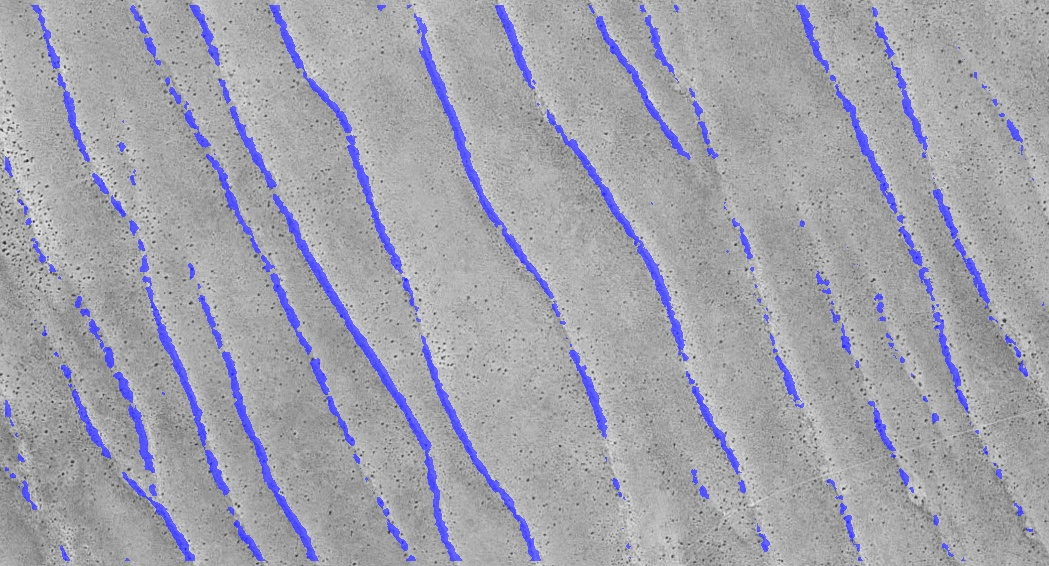
\includegraphics[scale=0.22]{Figures/ML/SVM/KalahariSVMResults1}
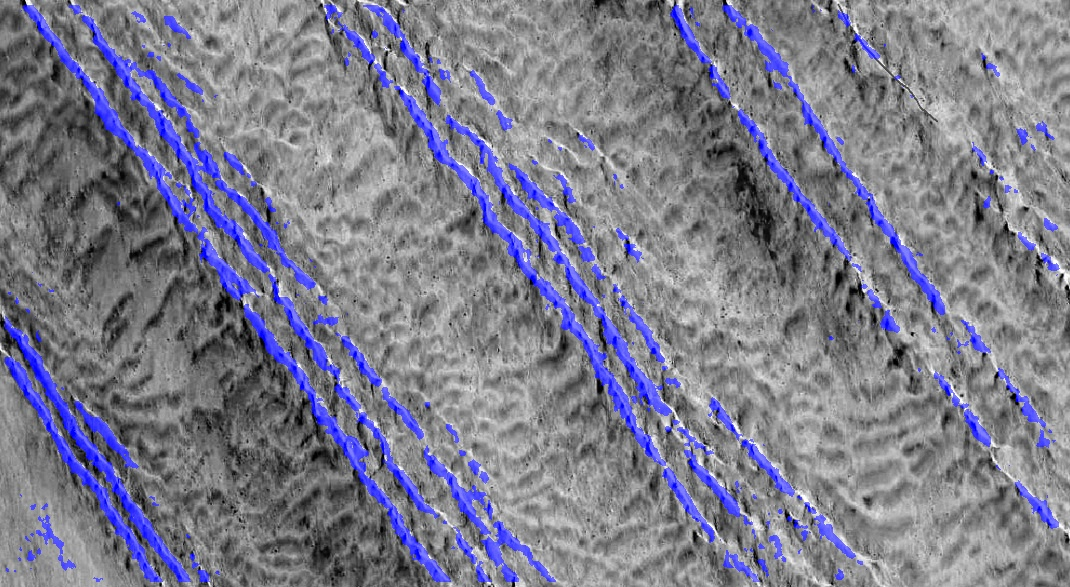
\includegraphics[scale=0.21]{Figures/ML/SVM/NamibSVMResults1}}
\par\end{centering}

\begin{centering}
\textcolor{black}{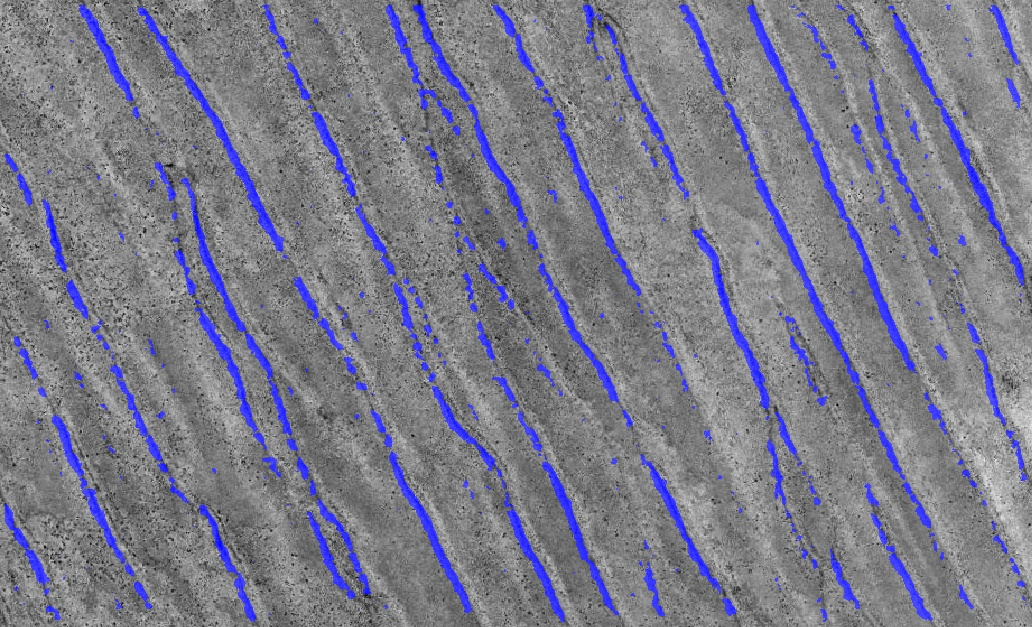
\includegraphics[scale=0.21]{Figures/ML/SVM/SimpsonSVMResults1}
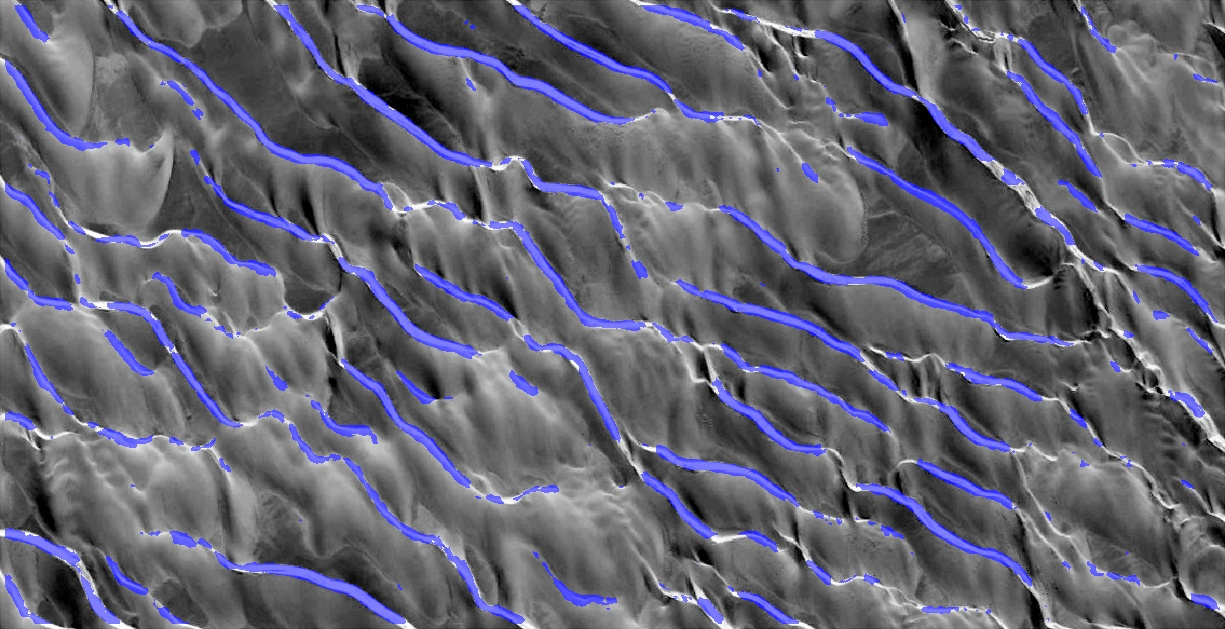
\includegraphics[scale=0.21]{Figures/ML/SVM/SkeletonCoastSVMResults1}}
\par\end{centering}

\begin{centering}
\textcolor{black}{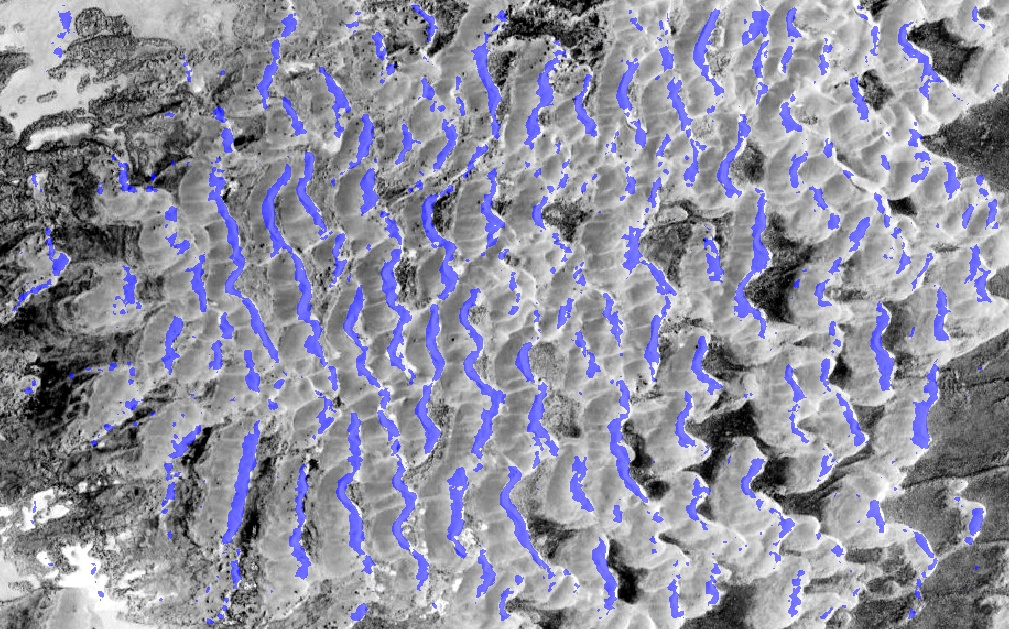
\includegraphics[scale=0.21]{Figures/ML/SVM/WDCSVMResults1}
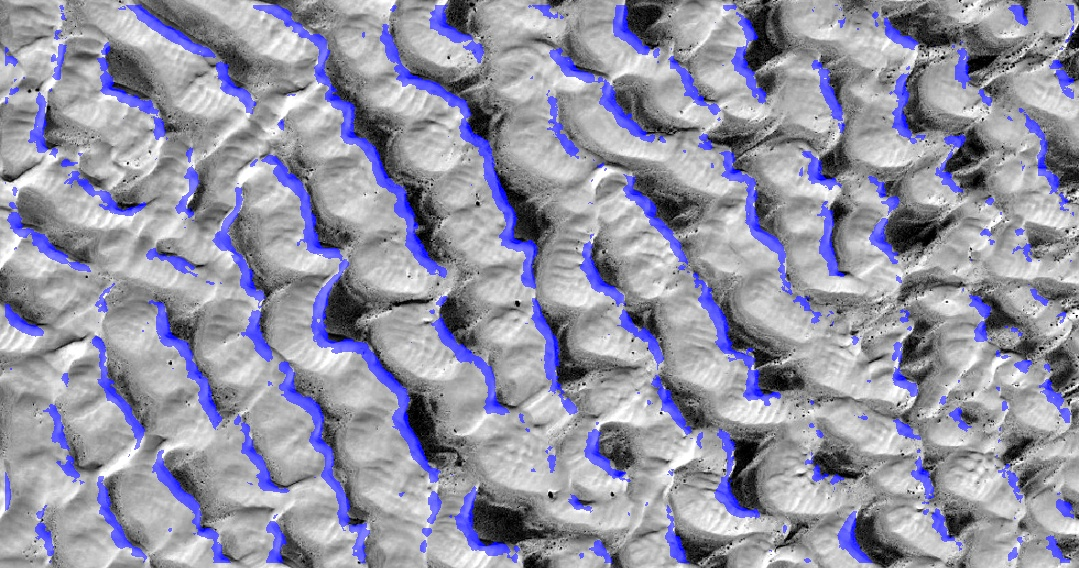
\includegraphics[scale=0.22]{Figures/ML/SVM/WhiteSandsSVMResults1}}
\par\end{centering}

\textcolor{black}{\protect\caption{\textcolor{red}{\label{fig:Results-of-the-SIFT-SVM}}\textcolor{black}{Results
of the SIFT features with the SVM }\textcolor{red}{classification
at each pixel location for each image}}
}
\end{figure*}


\textcolor{black}{}
\begin{figure*}
\begin{centering}
\textcolor{black}{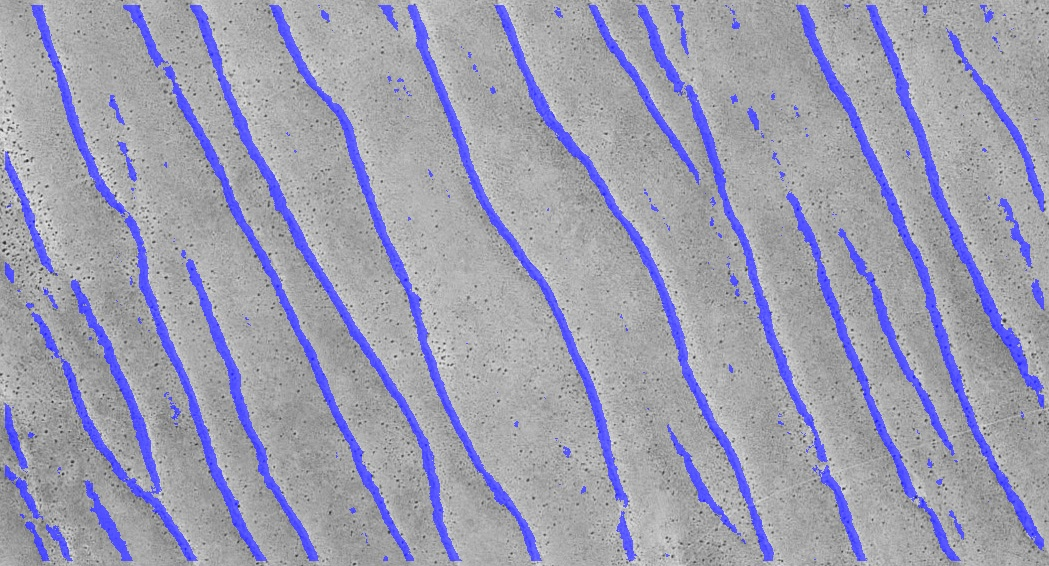
\includegraphics[scale=0.22]{Figures/ML/GBT/KalahariGBTResults1}
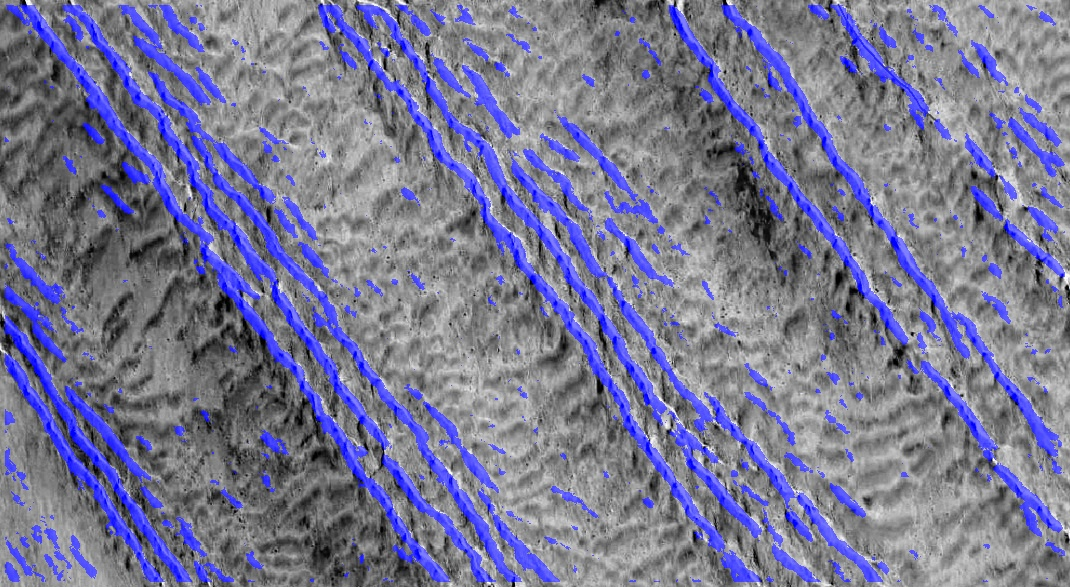
\includegraphics[scale=0.21]{Figures/ML/GBT/NamibGBTResults1}}
\par\end{centering}

\begin{centering}
\textcolor{black}{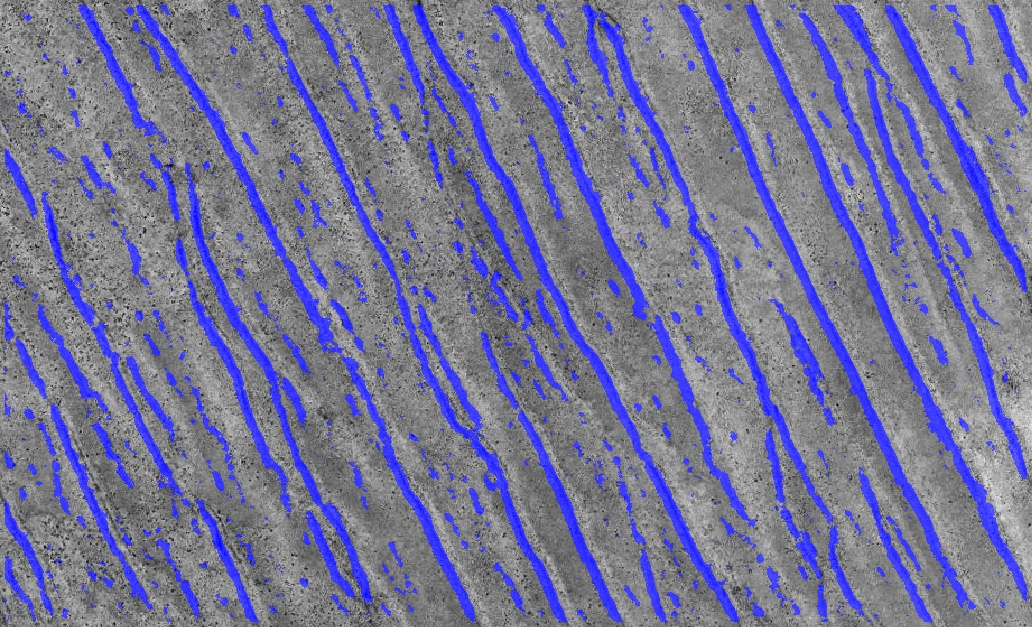
\includegraphics[scale=0.21]{Figures/ML/GBT/SimpsonGBTResults1}
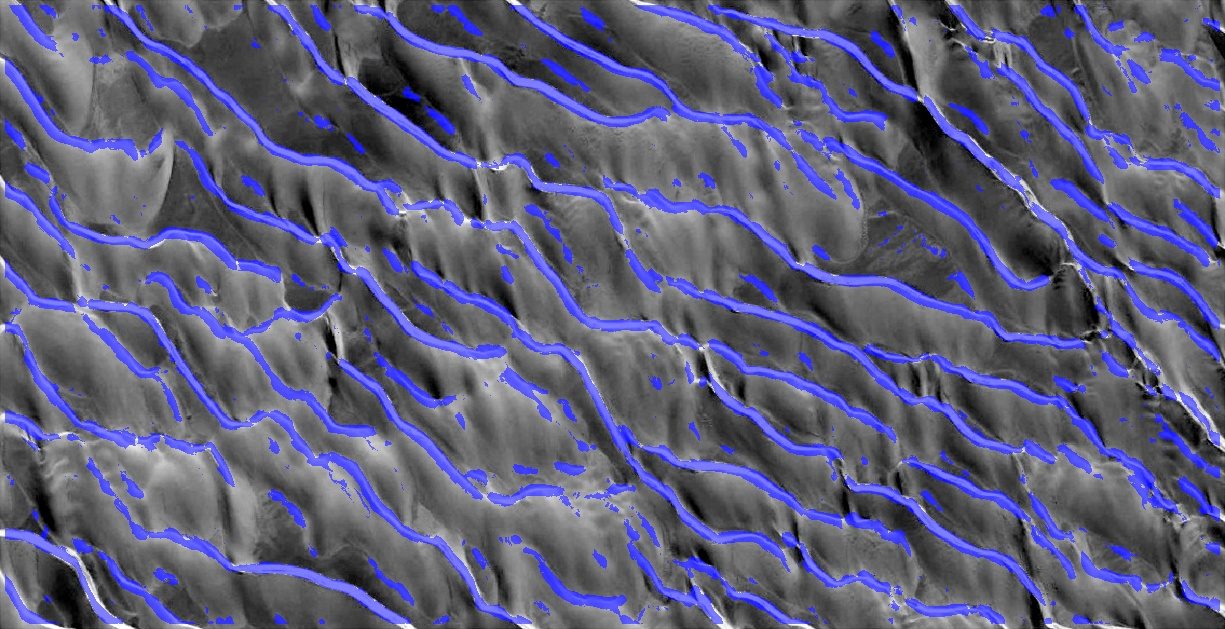
\includegraphics[scale=0.21]{Figures/ML/GBT/SkeletonCoastGBTResults1}}
\par\end{centering}

\begin{centering}
\textcolor{black}{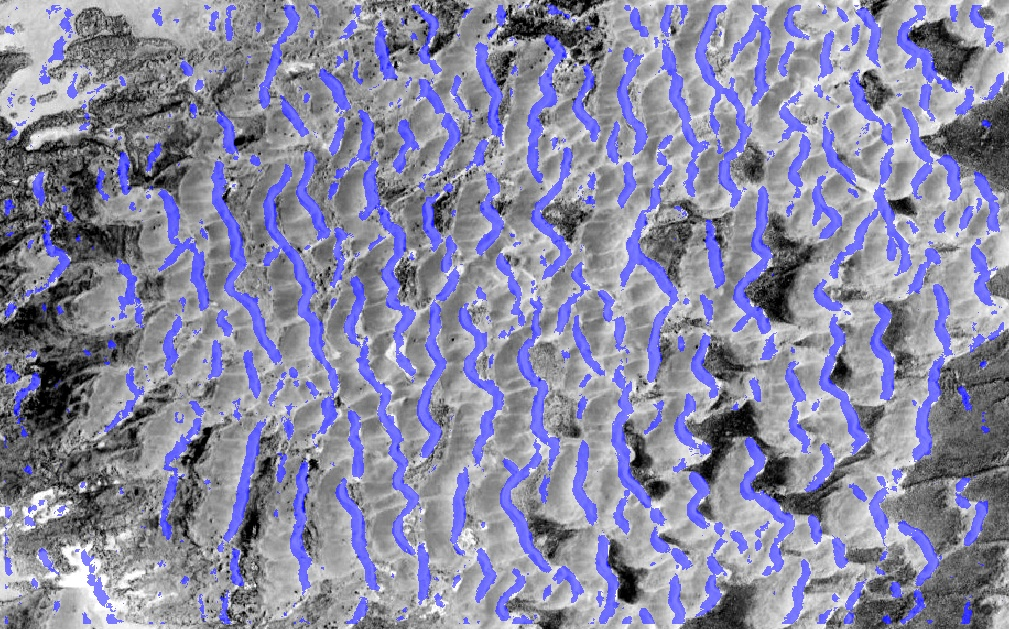
\includegraphics[scale=0.21]{Figures/ML/GBT/WDCGBTResults1}
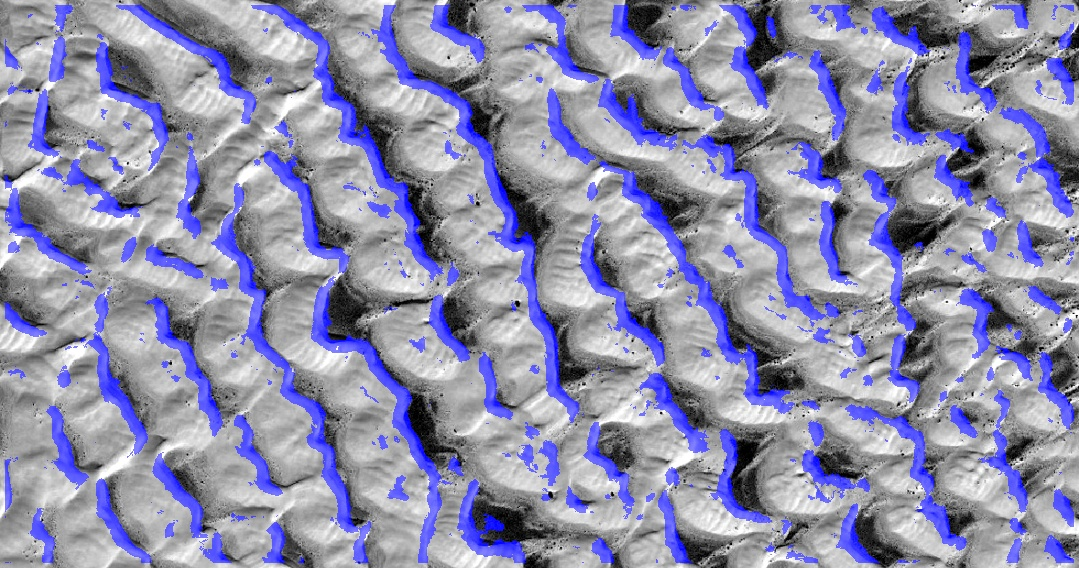
\includegraphics[scale=0.22]{Figures/ML/GBT/WhiteSandsGBTResults1}}
\par\end{centering}

\textcolor{black}{\protect\caption{\textcolor{red}{\label{fig:Results-of-the-SIFT-GBT}Results of the
SIFT features with the Gradient boosted tress classification at each
pixel location for each image}}
}
\end{figure*}



\paragraph*{\textcolor{black}{Response Image Thining Algorithm}}

\textcolor{black}{After training the classifier with the desired features,
each pixel in the image have their features computed and classified
using the trained classifier. The response output of the classifier
is typically a continuous value ranging in {[}-1, 1{]}, where -1 represents
a non-crestline pixel, and 1 is a crestline pixel. An example of the
output is shown in Figure \ref{fig:Response-image-thining} for the
Kalahari image using SIFT-GBT classifier.}

\textcolor{black}{The resulting classification produces thick lines,
which need to be thinned in order to produce the correct crestlines.
The algorithm on how this is done is shown in Figure \ref{fig:Recursive-thinning-algorithm}.
The algorithm is a recursive method to follow along a ridge starting
from a peak value in the response map. The ridge is recursively marked
as pixels are identified. The results, shown in Figure \ref{fig:Response-image-thining}(b),
tend to be quite noisy, therefore Gaussian smoothing is applied to
produce smoother curves (Figure \ref{fig:Response-image-thining}(c)).}

A better approach for thinning is proposed in (REFERENCE NEEDED!!!,
http://opencv-code.com/quick-tips/implementation-of-thinning-algorithm-in-opencv/).
Results are shown in Figure

The results are presented in Table \ref{tab:Results-of-the-1}.

\begin{figure}
\begin{centering}
\includegraphics[scale=0.22]{\string"Figures/Results_11_18_2015/Kalahari 3 image.jpg_response\string".jpg}
\par\end{centering}

\begin{centering}
(a)
\par\end{centering}

\begin{centering}
\includegraphics[scale=0.22]{\string"Figures/Results_11_18_2015/Kalahari 3 image.jpg_postproc_thin_results\string".jpg}
\par\end{centering}

\begin{centering}
(b)
\par\end{centering}

\begin{centering}
\includegraphics[scale=0.22]{\string"Figures/Results_11_18_2015/Kalahari 3 image.jpg_postproc_thin_results_smooth\string".jpg}
\par\end{centering}

\begin{centering}
(c)
\par\end{centering}

\protect\caption{\label{fig:Response-image-thining}\textcolor{red}{Response image
thining algorithm process results: (a) Response image of Kalahari
image with SIFT features and Gradient Boosted Trees Classifier (b)
Result of thinning algorithm applied to (a), (c) Post-processing to
smooth and remove noisy edges.}}
\end{figure}


\begin{figure*}
\begin{centering}
\includegraphics[scale=0.31]{\string"Figures/Skeletonization Algorithm\string".png}
\par\end{centering}

\protect\caption{\textcolor{red}{\label{fig:Recursive-thinning-algorithm}Recursive
thinning algorithm steps explained: On the first iteration, the algorithm
is initialized using the detected anchor pixels, and begin search
for each neighbor. Neighbors which are peaks along the ridge are used
as anchors for the iteration. This algorithm recursively follows the
ridge of the response images.} }


\end{figure*}


\begin{figure}
\begin{centering}
\includegraphics[scale=0.22]{\string"Figures/Results_12_02_2015/Method5/Kalahari 3 image.jpg_response\string".jpg}
\par\end{centering}

\begin{centering}
\textcolor{red}{\includegraphics[scale=0.22]{\string"Figures/Results_12_02_2015/Method5/Kalahari 3 image.jpg_postproc_threshold_results\string".jpg}}
\par\end{centering}

\begin{centering}
\textcolor{red}{\includegraphics[scale=0.22]{\string"Figures/Results_12_02_2015/Method5/Kalahari 3 image.jpg_postproc_thin_results\string".jpg}}
\par\end{centering}

\protect\caption{Results of the thinning algorithm (REFERENCE NEEDED!!!) from the response
results.}


\end{figure}



\subsection{\textcolor{red}{Dune Field Morphology Metrics }}

\textcolor{red}{With the reliable crest line data extracted, morphology
parameters of the target image can be computed. The desired properties
include crest line lenght, dune scale, distance between dune crests,
and other properties. TODO (more research on this later).}

\textcolor{red}{The most important metrics to compute are the average
spacing between dune crests and average orientation of the dune field.
The orientation can be computed by taking fitting lines to detected
crest-lines and averaging the orientations of all the lines. Since
in many cases, the crest-lines are not always linear, a crest-line
can be approximated by fitting many smaller line segments. Another
problem is that often the crest-lines are not single lines, and may
fork or split into other bifurcations, which will cause issues when
attempting to fit a single line to a crest-line. Also, these features
are interesting to study, and should be detected and extracted.}

\textcolor{red}{In order to solve these issues, the detected candidate
crest-lines need to be grouped into single line segments. An iterative
algorithm is used to sort the detection and group them into single
line segments. Grouping the detections into single segments will allow
to more easily approximate and fit lines to each part of the segment.
In figure \ref{fig:Grouping-Detections-into}, a sample test image
is used to validate the algorithm. The results are not perfect for
the time being since in many cases the algorithm appears to break
straight lines at split points. But, this is not as critical of an
issue for fitting line segments, and ultimately this will allow us
to detect these split points (TODO).}

\begin{figure*}
\begin{centering}
(a) 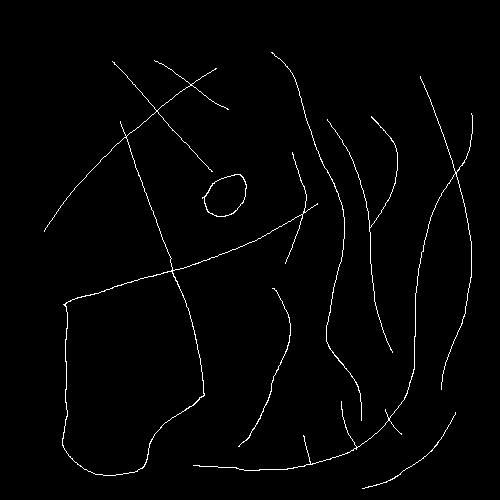
\includegraphics[scale=0.3]{Figures/Tests/testimage} (b) \includegraphics[scale=0.3]{Figures/Tests/SegmentationTest}
\par\end{centering}

\textcolor{red}{\protect\caption{\textcolor{red}{\label{fig:Grouping-Detections-into}Grouping Detections
into single line segments. (a) A example test images with many bifurcations
and splits. (b) Resulting groups.}}
}
\end{figure*}


\textcolor{red}{Once the groups have been found, each segment is approximated
with many lines. The metrics we are most interested in is the average
orientation of the dunes and the inter-dune distance. The average
orientation can easily be computed by averaging the orientation of
all the line segments detected. Once the average orientation has been
determined, the inter-dune distance can be computed by iteratively
counting the number of pixels between two crest-lines by searching
in straight lines perpendicular to the average orientation. This process
is illustrated in Figure \ref{fig:Computing-the-dune}.}

\begin{figure}
\begin{centering}
\includegraphics[scale=0.5]{Figures/Tests/DuneMetrics}
\par\end{centering}

\protect\caption{\label{fig:Computing-the-dune}\textcolor{red}{Computing the dune
metrics.}}


\end{figure}



\section{\textcolor{black}{Experiments}}

\textcolor{black}{Since the goal of this project is to automatically
segment dune crest lines, a dataset of images with labeled ground
truth is used to measure the accuracy of the dune detection algorithm.
The current dataset is a small sample set of six images taken from
different regions, at various scale and various illuminations. The
regions include: Kalahari, Namib, Simpson, Skeleton Coast, WDC, and
White Sands, as shown in figure \ref{fig:Dune-dataset-with}.}

\textcolor{black}{TODO.}

\textcolor{black}{}
\begin{figure*}
\begin{centering}
\textcolor{black}{(1)\includegraphics[scale=0.15]{\string"Figures/Datasets/Kalahari 3 image\string".jpg}
\includegraphics[scale=0.15]{\string"Figures/Datasets/Kalahari 3_gt\string".jpg}}
\par\end{centering}

\begin{centering}
\textcolor{black}{(2) \includegraphics[scale=0.15]{\string"Figures/Datasets/Namib 2 image\string".jpg}
\includegraphics[clip,scale=0.15]{\string"Figures/Datasets/Namib 2_gt\string".jpg}}
\par\end{centering}

\begin{centering}
\textcolor{black}{(3) \includegraphics[scale=0.15]{\string"Figures/Datasets/Simpson 1_image\string".jpg}
\includegraphics[clip,scale=0.15]{\string"Figures/Datasets/Simpson 1_gt\string".jpg}}
\par\end{centering}

\begin{centering}
\textcolor{black}{(4) \includegraphics[scale=0.15]{\string"Figures/Datasets/Skeleton Coast 3_image\string".jpg}
\includegraphics[clip,scale=0.15]{\string"Figures/Datasets/Skeleton Coast 3_gt\string".jpg}}
\par\end{centering}

\begin{centering}
\textcolor{black}{(5) \includegraphics[scale=0.15]{Figures/Datasets/WDC_1_image}
\includegraphics[scale=0.15]{Figures/Datasets/WDC_1_gt}}
\par\end{centering}

\begin{centering}
\textcolor{black}{(6) \includegraphics[scale=0.15]{\string"Figures/Datasets/White Sands_2_image\string".jpg}
\includegraphics[scale=0.15]{\string"Figures/Datasets/White Sands_2_gt\string".jpg}}
\par\end{centering}

\textcolor{black}{\protect\caption{\label{fig:Dune-dataset-with}\textcolor{red}{Training }Dune dataset
with corresponding dune crest line ground truth map. The images are
labeled as (1) Kalahari, (2) Namib, (3) Simpson, (4) Skeleton Coast,
(5) WDC, and (6) White Sands.}
}

\end{figure*}


\textcolor{black}{}
\begin{figure*}
\begin{centering}
\textcolor{black}{(1)\includegraphics[scale=0.14]{\string"Figures/Datasets/Kalahari 3 test\string".jpg}
\includegraphics[scale=0.14]{\string"Figures/Datasets/Kalahari 3 test_gt\string".png}}
\par\end{centering}

\begin{centering}
\textcolor{black}{(2) \includegraphics[scale=0.14]{\string"Figures/Datasets/Namib 2 test\string".jpg}
\includegraphics[clip,scale=0.14]{\string"Figures/Datasets/Namib 2 test gt\string".png}}
\par\end{centering}

\begin{centering}
\textcolor{black}{(3) \includegraphics[scale=0.14]{\string"Figures/Datasets/Simpson 1 test\string".jpg}
\includegraphics[clip,scale=0.14]{\string"Figures/Datasets/Simpson 1 test_gt\string".png}}
\par\end{centering}

\begin{centering}
\textcolor{black}{(4) \includegraphics[scale=0.14]{\string"Figures/Datasets/Skeleton Coast 3 test\string".jpg}
\includegraphics[clip,scale=0.14]{\string"Figures/Datasets/Skeleton Coast 3 test_gt\string".png}}
\par\end{centering}

\begin{centering}
\textcolor{black}{(5) \includegraphics[scale=0.14]{\string"Figures/Datasets/WCD-1 test\string".jpg}
\includegraphics[scale=0.14]{\string"Figures/Datasets/WCD-1 test_gt\string".png}}
\par\end{centering}

\begin{centering}
\textcolor{black}{(6) \includegraphics[scale=0.14]{\string"Figures/Datasets/White Sands 2 test\string".jpg}
\includegraphics[scale=0.14]{\string"Figures/Datasets/White Sands 2 test-gt\string".png}}
\par\end{centering}

\textcolor{black}{\protect\caption{\label{fig:test-Dune-dataset}\textcolor{red}{Test }Dune dataset with
corresponding dune crest line ground truth map. The images are labeled
as (1) Kalahari, (2) Namib, (3) Simpson, (4) Skeleton Coast, (5) WDC,
and (6) White Sands.}
}
\end{figure*}



\section{\textcolor{black}{\label{sec:Results}Results}}

\textcolor{black}{The dune line crest detector is applied to the labeled
benchmark images shown in figure \ref{fig:Dune-dataset-with}. The
results we are interested in for detection purposes are the true positives
(correctly detected dune lines) and false positive (segments that
are not dunes). The results are computed in a brute force manner:}
\begin{enumerate}
\item \textbf{\textcolor{black}{\uline{True Positive Rate}}}\textcolor{black}{:
The }\textcolor{black}{\emph{TPRs}}\textcolor{black}{{} are computed
by taking each ground truth pixel, and finding the nearest detected
dune segment pixel. If the distance between the nearest detected and
the ground truth is smaller than some error }\textcolor{black}{\emph{e}}\textcolor{black}{,
the ground truth is considered to be detected. The }\textcolor{black}{\emph{TP}}\textcolor{black}{{}
rate is then the number of correctly identified ground truth points,
over the total number of ground truth points.}
\item \textbf{\textcolor{black}{\uline{False Positive Rate}}}\textcolor{black}{:
The }\textcolor{black}{\emph{FPRs}}\textcolor{black}{{} are computed
by taking each detected dune candidate, and finding the nearest ground
truth point. If that distance is greater than some error }\textcolor{black}{\emph{e}}\textcolor{black}{,
then the detected dune candidate is a false positive. The }\textcolor{black}{\emph{FP}}\textcolor{black}{{}
rate is then expressed as the number of incorrectly detected dune
points over the total number of dune points detected.}
\end{enumerate}
\textcolor{black}{The }\textcolor{black}{\emph{TP}}\textcolor{black}{{}
and }\textcolor{black}{\emph{FP}}\textcolor{black}{{} rates are shown
in table \ref{tab:Results-of-the}. The results shown in figure \ref{fig:Dune-detection-results}
visually overlaps the ground truth with the dune detected.}

\textcolor{black}{}
\begin{sidewaystable*}
\begin{centering}
\textcolor{black}{}%
\begin{tabular}{|c|c|c|c|c|}
\hline 
\multirow{2}{*}{\textbf{\textcolor{black}{Method \#1}}} & \multicolumn{2}{c|}{\textbf{\textcolor{black}{Image Set A}}} & \multicolumn{2}{c|}{\textbf{\textcolor{black}{Image Set B}}}\tabularnewline
\cline{2-5} 
 & \textbf{\textcolor{black}{Precision}} & \textbf{\textcolor{black}{Recall}} & \textbf{\textcolor{black}{Precision}} & \textbf{\textcolor{black}{Recall}}\tabularnewline
\hline 
\textcolor{black}{Kalahari} & \textcolor{black}{0.2524} & \textcolor{black}{0.0545} & \textcolor{black}{0.2836} & \textcolor{black}{0.8777}\tabularnewline
\hline 
\textcolor{black}{Namib} & \textcolor{black}{0.5564} & \textcolor{black}{0.1482} & \textcolor{black}{0.2479} & \textcolor{black}{0.9606}\tabularnewline
\hline 
\textcolor{black}{Simpson} & \textcolor{black}{0.3941} & \textcolor{black}{0.6220} & \textcolor{black}{0.4482} & \textcolor{black}{0.1555}\tabularnewline
\hline 
\textcolor{black}{Skeleton Coast} & \textcolor{black}{0.4526} & \textcolor{black}{0.9906} & \textcolor{black}{0.4725} & \textcolor{black}{0.0692}\tabularnewline
\hline 
\textcolor{black}{WDC} & \textcolor{black}{0.5856} & \textcolor{black}{0.9538} & \textcolor{black}{0.3552} & \textcolor{black}{0.9738}\tabularnewline
\hline 
\textcolor{black}{White Sands} & \textcolor{black}{0.4386} & \textcolor{black}{0.9223} & \textcolor{black}{0.3168} & \textcolor{black}{0.9041}\tabularnewline
\hline 
\end{tabular}\textcolor{black}{{} }%
\begin{tabular}{|c|c|c|c|c|}
\hline 
\multirow{2}{*}{\textbf{\textcolor{black}{Method \#2}}} & \multicolumn{2}{c|}{\textbf{\textcolor{black}{Image Set A}}} & \multicolumn{2}{c|}{\textbf{\textcolor{black}{Image Set B}}}\tabularnewline
\cline{2-5} 
 & \textbf{\textcolor{black}{Precision}} & \textbf{\textcolor{black}{Recall}} & \textbf{\textcolor{black}{Precision}} & \textbf{\textcolor{black}{Recall}}\tabularnewline
\hline 
\textcolor{black}{Kalahari} & \textcolor{black}{-} & \textcolor{black}{-} & \textcolor{black}{-} & \textcolor{black}{-}\tabularnewline
\hline 
\textcolor{black}{Namib} & \textcolor{black}{-} & \textcolor{black}{-} & \textcolor{black}{-} & \textcolor{black}{-}\tabularnewline
\hline 
\textcolor{black}{Simpson} & \textcolor{black}{-} & \textcolor{black}{-} & \textcolor{black}{-} & \textcolor{black}{-}\tabularnewline
\hline 
\textcolor{black}{Skeleton Coast} & \textcolor{black}{-} & \textcolor{black}{-} & \textcolor{black}{-} & \textcolor{black}{-}\tabularnewline
\hline 
\textcolor{black}{WDC} & \textcolor{black}{-} & \textcolor{black}{-} & \textcolor{black}{-} & \textcolor{black}{-}\tabularnewline
\hline 
\textcolor{black}{White Sands} & \textcolor{black}{-} & \textcolor{black}{-} & \textcolor{black}{-} & \textcolor{black}{-}\tabularnewline
\hline 
\end{tabular}
\par\end{centering}

\begin{centering}
\textcolor{black}{}%
\begin{tabular}{|c|c|c|c|c|}
\hline 
\multirow{2}{*}{\textbf{\textcolor{black}{Method \#3}}} & \multicolumn{2}{c|}{\textbf{\textcolor{black}{Image Set A}}} & \multicolumn{2}{c|}{\textbf{\textcolor{black}{Image Set B}}}\tabularnewline
\cline{2-5} 
 & \textbf{\textcolor{black}{Precision}} & \textbf{\textcolor{black}{Recall}} & \textbf{\textcolor{black}{Precision}} & \textbf{\textcolor{black}{Recall}}\tabularnewline
\hline 
\textcolor{black}{Kalahari} & \textcolor{black}{0.9087} & \textcolor{black}{0.8093} & \textcolor{black}{0.6634} & \textcolor{black}{0.7255}\tabularnewline
\hline 
\textcolor{black}{Namib} & \textcolor{black}{0.6115} & \textcolor{black}{0.6617} & \textcolor{black}{0.46122} & \textcolor{black}{0.6829}\tabularnewline
\hline 
\textcolor{black}{Simpson} & \textcolor{black}{0.6992} & \textcolor{black}{0.4893} & \textcolor{black}{0.5219} & \textcolor{black}{0.0797}\tabularnewline
\hline 
\textcolor{black}{Skeleton Coast} & \textcolor{black}{0.5700} & \textcolor{black}{0.7489} & \textcolor{black}{0.5950} & \textcolor{black}{0.6476}\tabularnewline
\hline 
\textcolor{black}{WDC} & \textcolor{black}{0.6279} & \textcolor{black}{0.2532} & \textcolor{black}{0.3817} & \textcolor{black}{0.3734}\tabularnewline
\hline 
\textcolor{black}{White Sands} & \textcolor{black}{0.4763} & \textcolor{black}{0.4068} & \textcolor{black}{0.5622} & \textcolor{black}{0.6945}\tabularnewline
\hline 
\end{tabular}\textbf{\textcolor{black}{{} }}\textcolor{black}{}%
\begin{tabular}{|c|c|c|c|c|}
\hline 
\multirow{2}{*}{\textbf{\textcolor{black}{Method \#4}}} & \multicolumn{2}{c|}{\textbf{\textcolor{black}{Image Set A}}} & \multicolumn{2}{c|}{\textbf{\textcolor{black}{Image Set B}}}\tabularnewline
\cline{2-5} 
 & \textbf{\textcolor{black}{Precision}} & \textbf{\textcolor{black}{Recall}} & \textbf{\textcolor{black}{Precision}} & \textbf{\textcolor{black}{Recall}}\tabularnewline
\hline 
\textcolor{black}{Kalahari} & \textcolor{black}{0.6329} & \textcolor{black}{0.9730} & \textcolor{black}{0.5436} & \textcolor{black}{0.9042}\tabularnewline
\hline 
\textcolor{black}{Namib} & \textcolor{black}{0.5835} & \textcolor{black}{0.9811} & \textcolor{black}{0.3949} & \textcolor{black}{0.9511}\tabularnewline
\hline 
\textcolor{black}{Simpson} & \textcolor{black}{0.6450} & \textcolor{black}{0.6857} & \textcolor{black}{0.4676} & \textcolor{black}{0.8080}\tabularnewline
\hline 
\textcolor{black}{Skeleton Coast} & \textcolor{black}{0.6448} & \textcolor{black}{0.7767} & \textcolor{black}{0.6865} & \textcolor{black}{0.7560}\tabularnewline
\hline 
\textcolor{black}{WDC} & \textcolor{black}{0.7221} & \textcolor{black}{0.6571} & \textcolor{black}{0.4388} & \textcolor{black}{0.6843}\tabularnewline
\hline 
\textcolor{black}{White Sands} & \textcolor{black}{0.4703} & \textcolor{black}{0.3601} & \textcolor{black}{0.5270} & \textcolor{black}{0.6601}\tabularnewline
\hline 
\end{tabular}
\par\end{centering}

\begin{centering}
\textcolor{black}{}%
\begin{tabular}{|c|c|c|c|c|c|c|c|c|c|c|}
\hline 
\multirow{2}{*}{\textbf{\textcolor{red}{Method \#5}}} & \multicolumn{5}{c|}{\textbf{\textcolor{red}{Image Set A}}} & \multicolumn{5}{c}{\textbf{\textcolor{red}{Image Set B}}}\tabularnewline
\cline{2-11} 
 & \textbf{\textcolor{red}{Precision}} & \textbf{\textcolor{red}{Recall}} & \textcolor{red}{$\mathbf{\theta_{err}}$ }\textbf{\textcolor{red}{(degrees)}} & \textbf{\textcolor{red}{$\mathbf{\delta}_{\mathbf{err}}$ (pixels)}} & \textcolor{red}{$\mathbf{\overline{\delta_{err}}}$} & \textbf{\textcolor{red}{Precision}} & \textbf{\textcolor{red}{Recall}} & \textcolor{red}{$\mathbf{\theta_{err}}$}\textbf{\textcolor{red}{(degrees)}} & \textbf{\textcolor{red}{$\mathbf{\delta}_{\mathbf{err}}$(pixels)}} & \textcolor{red}{$\mathbf{\overline{\delta_{err}}}$}\tabularnewline
\hline 
\textcolor{red}{Kalahari} & \textcolor{red}{0.9379} & \textcolor{red}{0.9726} & \textcolor{red}{$0.2437\textdegree$} & \textcolor{red}{3.9228} & \textcolor{red}{0.0611} & \textcolor{red}{0.7694} & \textcolor{red}{0.9232} & \textcolor{red}{$1.5047\textdegree$} & \textcolor{red}{7.6993} & \textcolor{red}{0.1319}\tabularnewline
\hline 
\textcolor{red}{Namib} & \textcolor{red}{0.8491} & \textcolor{red}{0.9676} & \textcolor{red}{$8.0655\textdegree$} & \textcolor{red}{13.2756} & \textcolor{red}{0.2023} & \textcolor{red}{0.7867} & \textcolor{red}{0.8778} & \textcolor{red}{$2.8757\textdegree$} & \textcolor{red}{4.0135} & \textcolor{red}{0.0753}\tabularnewline
\hline 
\textcolor{red}{Simpson} & \textcolor{red}{0.9084} & \textcolor{red}{0.9249} & \textcolor{red}{$13.0593\textdegree$} & \textcolor{red}{8.3083} & \textcolor{red}{0.1391} & \textcolor{red}{0.7658} & \textcolor{red}{0.8398} & \textcolor{red}{$0.7329\textdegree$} & \textcolor{red}{2.4516} & \textcolor{red}{0.0458}\tabularnewline
\hline 
\textcolor{red}{Skeleton Coast} & \textcolor{red}{0.7632} & \textcolor{red}{0.9536} & \textcolor{red}{$0.0434\textdegree$} & \textcolor{red}{9.5747} & \textcolor{red}{0.1759} & \textcolor{red}{0.7938} & \textcolor{red}{0.9393} & \textcolor{red}{$1.4801\textdegree$} & \textcolor{red}{1.5155} & \textcolor{red}{0.0351}\tabularnewline
\hline 
\textcolor{red}{WDC} & \textcolor{red}{0.8981} & \textcolor{red}{0.8554} & \textcolor{red}{$1.9937\textdegree$} & \textcolor{red}{1.9692} & \textcolor{red}{0.0362} & \textcolor{red}{0.7558} & \textcolor{red}{0.8559} & \textcolor{red}{$2.1001\textdegree$} & \textcolor{red}{1.7801} & \textcolor{red}{0.0312}\tabularnewline
\hline 
\textcolor{red}{White Sands} & \textcolor{red}{0.9370} & \textcolor{red}{0.8784} & \textcolor{red}{$10.6052\textdegree$} & \textcolor{red}{4.3457} & \textcolor{red}{0.0562} & \textcolor{red}{0.8695} & \textcolor{red}{0.8001} & \textcolor{red}{$2.5835\textdegree$} & \textcolor{red}{7.8096} & \textcolor{red}{0.1389}\tabularnewline
\hline 
\end{tabular}
\par\end{centering}

\begin{centering}
\textcolor{black}{}%
\begin{tabular}{|c|c|c|c|c|c|c|c|c|c|c|}
\hline 
\multirow{2}{*}{\textbf{\textcolor{red}{Method \#5 Cross-Training}}} & \multicolumn{5}{c|}{\textbf{\textcolor{red}{Image Set A}}} & \multicolumn{5}{c}{\textbf{\textcolor{red}{Image Set B}}}\tabularnewline
\cline{2-11} 
 & \textbf{\textcolor{red}{Precision}} & \textbf{\textcolor{red}{Recall}} & \textcolor{red}{$\mathbf{\theta_{err}}$}\textbf{\textcolor{red}{{}
(degrees)}} & \textbf{\textcolor{red}{$\mathbf{\delta}_{\mathbf{err}}$ (pixels)}} & \textcolor{red}{$\mathbf{\overline{\delta_{err}}}$} & \textbf{\textcolor{red}{Precision}} & \textbf{\textcolor{red}{Recall}} & \textcolor{red}{$\mathbf{\theta_{err}}$ }\textbf{\textcolor{red}{(degrees)}} & \textbf{\textcolor{red}{$\mathbf{\delta}_{\mathbf{err}}$ (pixels)}} & \textcolor{red}{$\mathbf{\overline{\delta_{err}}}$}\tabularnewline
\hline 
\textcolor{red}{Kalahari} & \textcolor{red}{0.9258} & \textcolor{red}{0.9254} & \textcolor{red}{$0.4803\textdegree$} & \textcolor{red}{5.0142} & \textcolor{red}{0.0781} & \textcolor{red}{0.7300} & \textcolor{red}{0.8444} & \textcolor{red}{$1.0343\textdegree$} & \textcolor{red}{5.9187} & \textcolor{red}{0.1014}\tabularnewline
\hline 
\textcolor{red}{Namib} & \textcolor{red}{0.7942} & \textcolor{red}{0.9590} & \textcolor{red}{$2.8976\textdegree$} & \textcolor{red}{16.7863} & \textcolor{red}{0.2559} & \textcolor{red}{0.6637} & \textcolor{red}{0.8634} & \textcolor{red}{$9.5319\textdegree$} & \textcolor{red}{2.4645} & \textcolor{red}{0.0462}\tabularnewline
\hline 
\textcolor{red}{Simpson} & \textcolor{red}{0.8491} & \textcolor{red}{0.7854} & \textcolor{red}{$13.938\textdegree$} & \textcolor{red}{9.0225} & \textcolor{red}{0.1511} & \textcolor{red}{0.7375} & \textcolor{red}{0.7579} & \textcolor{red}{$0.2434\textdegree$} & \textcolor{red}{2.7176} & \textcolor{red}{0.0507}\tabularnewline
\hline 
\textcolor{red}{Skeleton Coast} & \textcolor{red}{0.5768} & \textcolor{red}{0.9096} & \textcolor{red}{$10.4224\textdegree$} & \textcolor{red}{18.6251} & \textcolor{red}{0.3423} & \textcolor{red}{0.6135} & \textcolor{red}{0.8967} & \textcolor{red}{$7.7421\textdegree$} & \textcolor{red}{8.3473} & \textcolor{red}{0.1932}\tabularnewline
\hline 
\textcolor{red}{WDC} & \textcolor{red}{0.9315} & \textcolor{red}{0.6155} & \textcolor{red}{$12.7138\textdegree$} & \textcolor{red}{11.1957} & \textcolor{red}{0.2058} & \textcolor{red}{0.8585} & \textcolor{red}{0.5771} & \textcolor{red}{$15.8434\textdegree$} & \textcolor{red}{21.4145} & \textcolor{red}{0.3757}\tabularnewline
\hline 
\textcolor{red}{White Sands} & \textcolor{red}{0.9374} & \textcolor{red}{0.6431} & \textcolor{red}{$11.0979\textdegree$} & \textcolor{red}{15.9853} & \textcolor{red}{0.2069} & \textcolor{red}{0.7909} & \textcolor{red}{0.3973} & \textcolor{red}{$1.2744\textdegree$} & \textcolor{red}{53.3311} & \textcolor{red}{0.9489}\tabularnewline
\hline 
\end{tabular}
\par\end{centering}

\begin{centering}
\textcolor{black}{Old results}
\par\end{centering}

\begin{centering}
\textcolor{black}{}%
\begin{tabular}{|c|c|c|c|c|c|c|c|c|}
\hline 
\multirow{2}{*}{\textbf{\textcolor{black}{Images}}} & \multicolumn{2}{c|}{\textbf{\textcolor{black}{Method \#1}}} & \multicolumn{2}{c|}{\textbf{\textcolor{black}{Method \#2 (K-M)}}} & \multicolumn{2}{c|}{\textbf{\textcolor{black}{Method \#2 (HoG)}}} & \multicolumn{2}{c|}{\textbf{\textcolor{black}{Method \#3}}}\tabularnewline
\cline{2-9} 
 & \textbf{\textcolor{black}{\emph{TPR}}} & \textbf{\textcolor{black}{\emph{FPR}}} & \textbf{\textcolor{black}{\emph{TPR}}} & \textbf{\textcolor{black}{\emph{FPR}}} & \textbf{\textcolor{black}{\emph{TPR}}} & \textbf{\textcolor{black}{\emph{FPR}}} & \textbf{\textcolor{black}{\emph{TPR}}} & \textbf{\textcolor{black}{\emph{FPR}}}\tabularnewline
\hline 
\hline 
\textcolor{black}{Kalahari} & \textcolor{black}{0.7094} & \textbf{\textcolor{black}{0.2178}} & \textcolor{black}{0.9396} & \textcolor{black}{0.2495} & \textbf{\textcolor{black}{0.9852}} & \textcolor{black}{0.7155} & \textcolor{black}{0.9239} & \textcolor{black}{0.5229}\tabularnewline
\hline 
\textcolor{black}{Namib} & \textcolor{black}{0.7493} & \textcolor{black}{0.6026} & \textcolor{black}{0.9281} & \textbf{\textcolor{black}{0.4924}} & \textbf{\textcolor{black}{0.9626}} & \textcolor{black}{0.6850} & \textcolor{black}{0.8591} & \textcolor{black}{0.7290}\tabularnewline
\hline 
\textcolor{black}{Simpson} & \textcolor{black}{0.1364} & \textcolor{black}{0.6512} & \textcolor{black}{0.7464} & \textbf{\textcolor{black}{0.4979}} & \textbf{\textcolor{black}{0.8977}} & \textcolor{black}{0.6478} & \textcolor{black}{0.4968} & \textcolor{black}{0.6979}\tabularnewline
\hline 
\textcolor{black}{Skeleton Coast} & \textbf{\textcolor{black}{0.8033}} & \textcolor{black}{0.3253} & \textcolor{black}{0.7605} & \textbf{\textcolor{black}{0.1517}} & \textcolor{black}{0.8187} & \textcolor{black}{0.2178} & \textbf{\textcolor{black}{0.9221}} & \textcolor{black}{0.4461}\tabularnewline
\hline 
\textcolor{black}{WDC} & \textcolor{black}{0.5581} & \textbf{\textcolor{black}{0.3731}} & \textcolor{black}{0.5111} & \textcolor{black}{0.4849} & \textcolor{black}{0.7478} & \textcolor{black}{0.5399} & \textcolor{black}{0.7005} & \textcolor{black}{0.5819}\tabularnewline
\hline 
\textcolor{black}{White Sands} & \textcolor{black}{0.2614} & \textcolor{black}{0.6926} & \textbf{\textcolor{black}{0.6231}} & \textbf{\textcolor{black}{0.4762}} & \textcolor{black}{0.7634} & \textcolor{black}{0.5740} & \textcolor{black}{0.3889} & \textcolor{black}{0.8257}\tabularnewline
\hline 
\end{tabular}
\par\end{centering}

\begin{centering}
\textcolor{black}{}%
\begin{tabular}{|c|c|c|}
\hline 
\multirow{2}{*}{\textbf{\textcolor{black}{Images}}} & \multicolumn{2}{c|}{\textbf{\textcolor{black}{Method \#4 {*}{*}{*}}}}\tabularnewline
\cline{2-3} 
 & \textbf{\textcolor{black}{\emph{TPR}}} & \textbf{\textcolor{black}{\emph{FPR}}}\tabularnewline
\hline 
\hline 
\textcolor{black}{Kalahari} & \textcolor{black}{0.9370} & \textcolor{black}{0.3678}\tabularnewline
\hline 
\textcolor{black}{Namib} & \textcolor{black}{0.9883} & \textcolor{black}{0.6066}\tabularnewline
\hline 
\textcolor{black}{Simpson} & \textcolor{black}{0.5697} & \textcolor{black}{0.6677}\tabularnewline
\hline 
\textcolor{black}{Skeleton Coast} & \textcolor{black}{0.9935} & \textcolor{black}{0.2972}\tabularnewline
\hline 
\textcolor{black}{WDC} & \textcolor{black}{0.9302} & \textcolor{black}{0.2956}\tabularnewline
\hline 
\textcolor{black}{White Sands} & \textcolor{black}{0.6429} & \textcolor{black}{0.6420}\tabularnewline
\hline 
\end{tabular}
\par\end{centering}

\textcolor{black}{\protect\caption{\textcolor{red}{\label{tab:Results-of-the}Results of the dune detection
algorithms for the benchmark dataset using a value of }\textcolor{red}{\emph{e}}\textcolor{red}{{}
= 5 pixels. Method \#2 used $R=0.1$, {*}{*}{*} Because locatization
of Method \#4 is not as good, we use }\textcolor{red}{\emph{e}}\textcolor{red}{{}
= 10 pixels. For Method \#5, the ``Cross-Training'' is done by using
the training data from all six datasets to train the classifier.}}
}
\end{sidewaystable*}


\textcolor{red}{The metrics were calculated on both the resulting
crest-line and on the ground truth using the same process described
above. The error results reported in Table \ref{tab:Results-of-the},
are the following: }
\begin{itemize}
\item \textcolor{red}{The average orientation error: $\mathbf{\mathbf{\mathbf{\theta_{err}}=\mathbf{\left\Vert \theta_{det}-\theta_{true}\right\Vert }}}$}
\item \textcolor{red}{The average inter-dune distance: $\mathbf{\mathbf{\delta}_{err}=}\left\Vert \mathbf{\delta_{det}-\delta_{true}}\right\Vert $}
\item \textcolor{red}{The normalized inter-dune distance error: $\mathbf{\overline{\delta_{err}}}=\mathbf{\frac{\mathbf{\delta}_{err}}{\delta_{true}}}$
.}
\end{itemize}
\textcolor{black}{}
\begin{figure}
\begin{centering}
\textcolor{black}{(1)}
\par\end{centering}

\begin{centering}
\textcolor{black}{\includegraphics[scale=0.01]{\string"Figures/Kalahari Results001\string".jpg}}
\par\end{centering}

\begin{centering}
\textcolor{black}{(2)}
\par\end{centering}

\begin{centering}
\textcolor{black}{\includegraphics[scale=0.01]{\string"Figures/Simpson Results001\string".jpg}}
\par\end{centering}

\begin{centering}
\textcolor{black}{(3)}
\par\end{centering}

\begin{centering}
\textcolor{black}{\includegraphics[scale=0.01]{\string"Figures/Skeleton Coast Results001\string".jpg}}
\par\end{centering}

\textcolor{black}{\protect\caption{\label{fig:Dune-detection-results}Dune detection results (red) compared
to the ground truth (green), overall is shown in yellow. Shown are
results for (1) Kalahari, (2) Simpson, and (3) Skeleton Coast benchmark
images }
}

\end{figure}


\textcolor{black}{}
\begin{figure*}
\begin{centering}
\textcolor{black}{(a)}
\par\end{centering}

\begin{centering}
\textcolor{black}{\includegraphics[scale=0.01]{Figures/WatershedDuneSegments}}
\par\end{centering}

\begin{centering}
\textcolor{black}{(b)}
\par\end{centering}

\begin{centering}
\textcolor{black}{\includegraphics[scale=0.3]{Figures/Method4Results}}
\par\end{centering}

\begin{centering}
\textcolor{black}{(c)}
\par\end{centering}

\begin{centering}
\textcolor{black}{\includegraphics[scale=0.35]{Figures/Method4Results_2}}
\par\end{centering}

\textcolor{black}{\protect\caption{\textcolor{black}{\label{fig:Dune-Crestline-detection}(a) Dune Crestline
detection using Watershed Algorithm (Method \#3). (b) and (c) Results
of the Gradient Direction approach (Method \#4) with TP in green and
FP in red, for Skeleton Coast and WDC.}\textcolor{red}{{} }}
}

\end{figure*}


\begin{figure*}
\begin{centering}
\textcolor{black}{(a)}
\par\end{centering}

\begin{centering}
\includegraphics[scale=0.22]{\string"Figures/Results_12_02_2015/Method5/Kalahari 3 test.jpg_response\string".jpg}
\includegraphics[scale=0.22]{\string"Figures/Results_12_02_2015/Method5/Kalahari 3 test.jpg_results\string".jpg}
\par\end{centering}

\begin{centering}
\textcolor{black}{(b)}
\par\end{centering}

\begin{centering}
\includegraphics[scale=0.22]{\string"Figures/Results_12_02_2015/Method5/Namib 2 test.jpg_response\string".jpg}
\includegraphics[scale=0.22]{\string"Figures/Results_12_02_2015/Method5/Namib 2 test.jpg_results\string".jpg}
\par\end{centering}

\begin{centering}
\textcolor{black}{(c)}
\par\end{centering}

\begin{centering}
\includegraphics[scale=0.22]{\string"Figures/Results_12_02_2015/Method5/Simpson 1 test.jpg_response\string".jpg}
\includegraphics[scale=0.22]{\string"Figures/Results_12_02_2015/Method5/Simpson 1 test.jpg_results\string".jpg}
\par\end{centering}

\textcolor{red}{\protect\caption{\textcolor{red}{\label{fig:Dune-Crestline-detection-Method5}Results
of crestline detection using machine learning approach (Method \#5),
using SIFT-GBT classifier. Colors Scheme - Green: Correctly detected
crestline, Red: false positive, Blue: Correctly identified ground
truth point, Yellow: False negative. (a) Kalahari test image results,
(b) Namib test image, (c) Simpson test image}}
}
\end{figure*}


\begin{figure*}
\begin{centering}
(a)
\par\end{centering}

\begin{centering}
\includegraphics[scale=0.2]{\string"Figures/Results_12_02_2015/Method5/Skeleton Coast 3 test.jpg_response\string".jpg}
\includegraphics[scale=0.2]{\string"Figures/Results_12_02_2015/Method5/Skeleton Coast 3 test.jpg_results\string".jpg}
\par\end{centering}

\begin{centering}
(b)
\par\end{centering}

\begin{centering}
\includegraphics[scale=0.22]{\string"Figures/Results_12_02_2015/Method5/WCD-1 test.jpg_response\string".jpg}
\includegraphics[scale=0.22]{\string"Figures/Results_12_02_2015/Method5/WCD-1 test.jpg_results\string".jpg}
\par\end{centering}

\begin{centering}
(c)
\par\end{centering}

\begin{centering}
\includegraphics[scale=0.22]{\string"Figures/Results_12_02_2015/Method5/White Sands 2 test.jpg_response\string".jpg}
\includegraphics[scale=0.22]{\string"Figures/Results_12_02_2015/Method5/White Sands 2 test.jpg_results\string".jpg}
\par\end{centering}

\protect\caption{\label{fig:Continued-results-of}\textcolor{red}{Continued results
of crestline detection using machine learning approach: }}


\end{figure*}


\begin{figure*}
\begin{centering}
\includegraphics[scale=0.35]{Figures/Results_11_18_2015/window_size_results_test}
\par\end{centering}

\protect\caption{\textcolor{red}{\label{fig:Results-of-varying}Results of varying
the window size of features for machine learning approach method \#5
(SIFT-GBT)}.}
\end{figure*}


\textcolor{black}{In Figure \ref{fig:Precision-Recall-curves-for},
the Precision-Recall curves are shown for the various algorithms,
by varying the parameters. The P-R curves are computed as shown in
\cite{Relationship-between-precision-recall-roc-curves}, as follows:}

\textcolor{black}{
\[
Recall=\frac{TP}{TP+FN}
\]
}

\textcolor{black}{
\[
Precision=\frac{TP}{TP+FP}
\]
}

\textcolor{black}{}
\begin{figure*}
\begin{centering}
\textcolor{black}{(a)}
\par\end{centering}

\begin{centering}
\textcolor{black}{\includegraphics[scale=0.25]{Figures/gnuplots/eb_data_intensity1}}
\par\end{centering}

\begin{centering}
\textcolor{black}{(b)}
\par\end{centering}

\begin{centering}
\textcolor{black}{\includegraphics[scale=0.25]{Figures/gnuplots/eb_data_gradient2}}
\par\end{centering}

\begin{centering}
\textcolor{black}{\protect\caption{\textcolor{red}{\label{fig:Precision-Recall-curves-for}}\textcolor{black}{Precision-Recall
curves for the various algoritms used. (a) P-R curve for the Edge-Based
approach by varying the }\textcolor{black}{\emph{R}}\textcolor{black}{{}
parameter for intensity values. (b) P-R curve computed by shifting
the detected crestlines to the nearest gradient magnitude peak. }}
}
\par\end{centering}

\centering{}
\end{figure*}



\section{\textcolor{black}{Conclusion}}

\textcolor{black}{TODO.}

\textcolor{black}{\bibliographystyle{plain}
\addcontentsline{toc}{section}{\refname}\nocite{*}
\bibliography{references}
}
\end{document}
